\documentclass[../../../main.tex]{subfiles}

\begin{document}

\section{Wireframe}\label{s:wireframe}
Abbiamo realizzato i wireframe utilizzando il software \textit{Balsamiq}: per giungere alla loro versione finale sono state necessarie molte iterazioni.\\
Nelle sezioni che seguono, presentiamo ciascun wireframe, argomentando le scelte progettuali e le riflessioni alla loro base.

\subsection{Header e footer}\label{ss:header-e-footer}
Ogni schermata possiede un header nella parte superiore e uno footer, comune ovunque, nella parte inferiore: gli header variano in base alle necessità della schermata, come illustrato nelle figure seguenti.

\paragraph{Header}\mbox{}\\
\begin{figure}[H]
    \centering
    
\includegraphics[width=1\columnwidth]{wireframes/new-header-una-data}
    \caption{Header di ``Panoramica'' e ``Confronto fra regioni''.}
    \label{fig:header-una-data}
\end{figure}

\begin{figure}[H]
    \centering
    
\includegraphics[width=1\columnwidth]{wireframes/new-header-una-data-range}
    \caption{Header di ``Distribuzione su dati anagrafici''.}
    \label{fig:header-una-data-range}
\end{figure}

\begin{figure}[H]
    \centering
    
\includegraphics[width=1\columnwidth]{wireframes/new-header-due-date}
    \caption{Header di ``Analisi di periodi''.}
    \label{fig:header-due-date}
\end{figure}
\noindent
Gli elementi che compaiono nell'header, partendo da destra, sono:
\begin{itemize}
    \item logo del DPC;
    \item titolo e sottotitolo della dashboard;
    \item pulsante per aprire il menù per selezionare quali widget visualizzare;
    \item pulsante per ottenere un link condivisibile della dashboard e dell'organizzazione delle schermate (Figura \ref{fig:box-condividi});
    \item selettore di date (due in Figura \ref{fig:header-due-date}) composto da:
    \begin{itemize}
        \item un bottone con un'icona di una freccia a sinistra per passare al giorno precedente a quello selezionato;
        \item un bottone per aprire il widget di selezione della data (Figura \ref{fig:selettore-data-singola} e Figura \ref{fig:selettore-range-date});
        \item un bottone con un'icona di una freccia a destra per passare al giorno successivo a quello selezionato (nel caso in cui il giorno selezionato sia quello corrente, questo bottone è disabilitato);
    \end{itemize}
\end{itemize}

\begin{figure}[H]
    \begin{subfigure}[b]{0.5\textwidth}
        \centering
        
\includegraphics[trim= 0 0 5 0, clip, width=0.4\textwidth]{wireframes/selettore-data-singola}
        \caption{Pulsante per aprire il widget per selezionare\\ una data singola.}\label{fig:selettore-data-singola}
    \end{subfigure}
\hfill
    \begin{subfigure}[b]{0.5\textwidth}
        \centering
        
\includegraphics[width=0.75\textwidth]{wireframes/selettore-range-date}
        \caption{Pulsante per aprire il widget per selezionare\\un range di date.}\label{fig:selettore-range-date}
    \end{subfigure}
    \caption{Pulsanti per aprire i widget per selezionare una data o un range di date.}
\end{figure}
\noindent
Alla prima visita della dashboard viene richiesto di abilitare la ricezione di notifiche: se accettata l'utente potrà ricevere una notifica di aggiornamento dei dati del giorno corrente.
\begin{figure}[H]
    \centering
    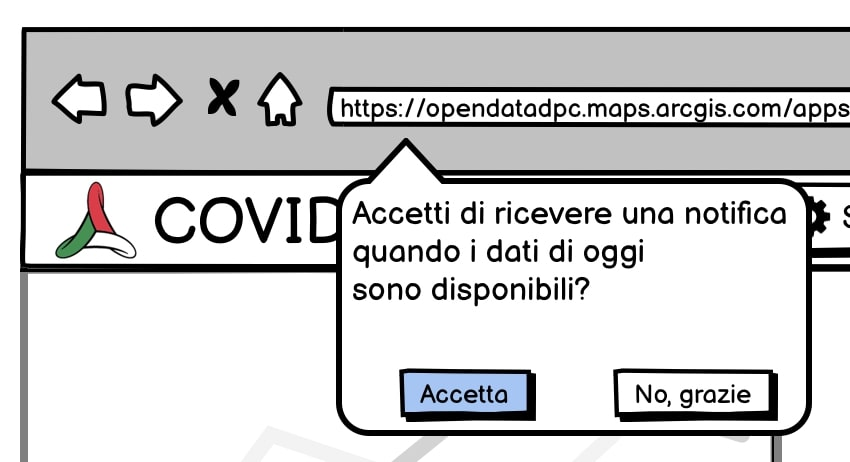
\includegraphics[width=0.3\columnwidth]{wireframes/richiesta-notifiche}
    \caption{Tooltip per richiedere l'abilitazione delle notifiche.}\label{fig:richiesta-notifiche}
\end{figure}
\noindent
\`E possibile condividere l'organizzazione della dashboard inviando il link ottenibile premendo il pulsante ``Condividi'' (Figura \ref{fig:box-condividi}).
\begin{figure}[H]
    \centering
    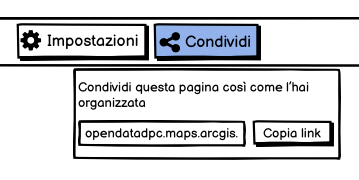
\includegraphics[width=0.3\columnwidth]{wireframes/box-condividi}
    \caption{Tooltip per ottenere il link condivisibile della dashboard.}\label{fig:box-condividi}
\end{figure}


\begin{bclogo}{Iterazioni sull'header}
Modifiche intercorse, nelle varie iterazioni, sull'header:
\begin{itemize}
    \item è stato aggiunto un bottone dall'etichetta ``Impostazioni'', al cui click compare una lista di metriche che l'utente può trascinare nella schermata: nelle prime versioni, la selezione di metriche diverse era resa possibile da bottoni presenti in ogni componente grafica con un'icona a ghiera, il che appesantiva notevolmente l'interfaccia. Il suo nome è stato cambiato da ``Seleziona metriche'' a ``Impostazioni'' dopo aver intervistato dei giornalisti i quali hanno espresso la loro difficoltà nel capire a cosa servisse, a prima vista, quel pulsante;
    \item i pulsanti per condividere e caricare (inizialmente separati) sono stati sostituiti da un unico pulsante ``Condividi'' per maggior chiarezza;
    \item sono stati cambiati i nomi delle schermate, nella direzione di una chiarezza maggiore;
    \item trasformazione delle icone di controllo del calendario in bottoni, per renderne più chiara la natura interattiva;
\end{itemize}
\begin{figure}[H]
    \centering
    
\includegraphics[width=1\columnwidth]{wireframes/header-vecchio}
    \caption{Prima versione dell'header.}\label{fig:header-vecchio}
\end{figure}
\begin{figure}[H]
    \centering
    
\includegraphics[width=1\columnwidth]{wireframes/header-una-data}
    \caption{Seconda versione dell'header.}\label{fig:header-finale}
\end{figure}
\begin{figure}[H]
    \centering
    
\includegraphics[width=1\columnwidth]{wireframes/new-header-una-data}
    \caption{Versione finale dell'header.}\label{fig:new-header-finale}
\end{figure}
\end{bclogo}

\paragraph{Seleziona metriche}\mbox{}\\
Il pulsante ``Impostazioni'' è stato aggiunto per permettere all'utilizzatore della dashboard di selezionare quali metriche visualizzare all'interno della schermata. Al suo click compare una lista (Figura \ref{fig:seleziona-metriche}) con tutte le metriche disponibili per quella schermata: l'utente può trascinare una metrica dalla lista all'interno della schermata e rilasciarla in una posizione compatibile andando così a sostituire una delle metriche presenti; mentre l'utente sta trascinando una metrica, le posizioni compatibili vengono evidenziate sull'interfaccia in quanto le uniche a colori e con una bordo ben marcato attorno.\\
Le metriche già presenti all'interno della schermata, indicate da una spunta (\checkmark), non sono trascinabili all'interno della schermata: nel caso l'utente tenti di trascinarle ugualmente, viene notificato che l'operazione non è permessa.\\
In caso l'utilizzatore della dashboard clicchi semplicemente su una metrica invece di selezionarla e trascinarla, compare un tooltip che spiega il funzionamento dell'interazione (Figura \ref{fig:seleziona-metriche-tooltip}).\\
\`E inoltre presente il pulsante ``Ripristina le metriche di default'' per ripristinare la schermata alle metriche di default.

\begin{figure}[H]
    \begin{subfigure}[b]{0.5\textwidth}
        \centering
        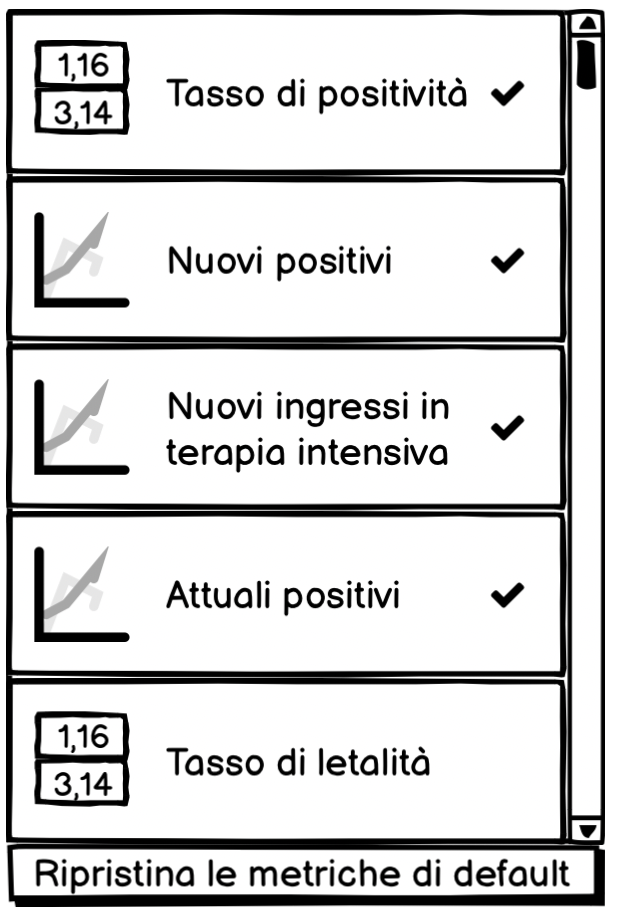
\includegraphics[width=0.3\textwidth]{wireframes/seleziona-metriche}
        \caption{Menù di selezione delle metriche.}
        \label{fig:seleziona-metriche}
    \end{subfigure}
\hfill
    \begin{subfigure}[b]{0.5\textwidth}
        \centering
        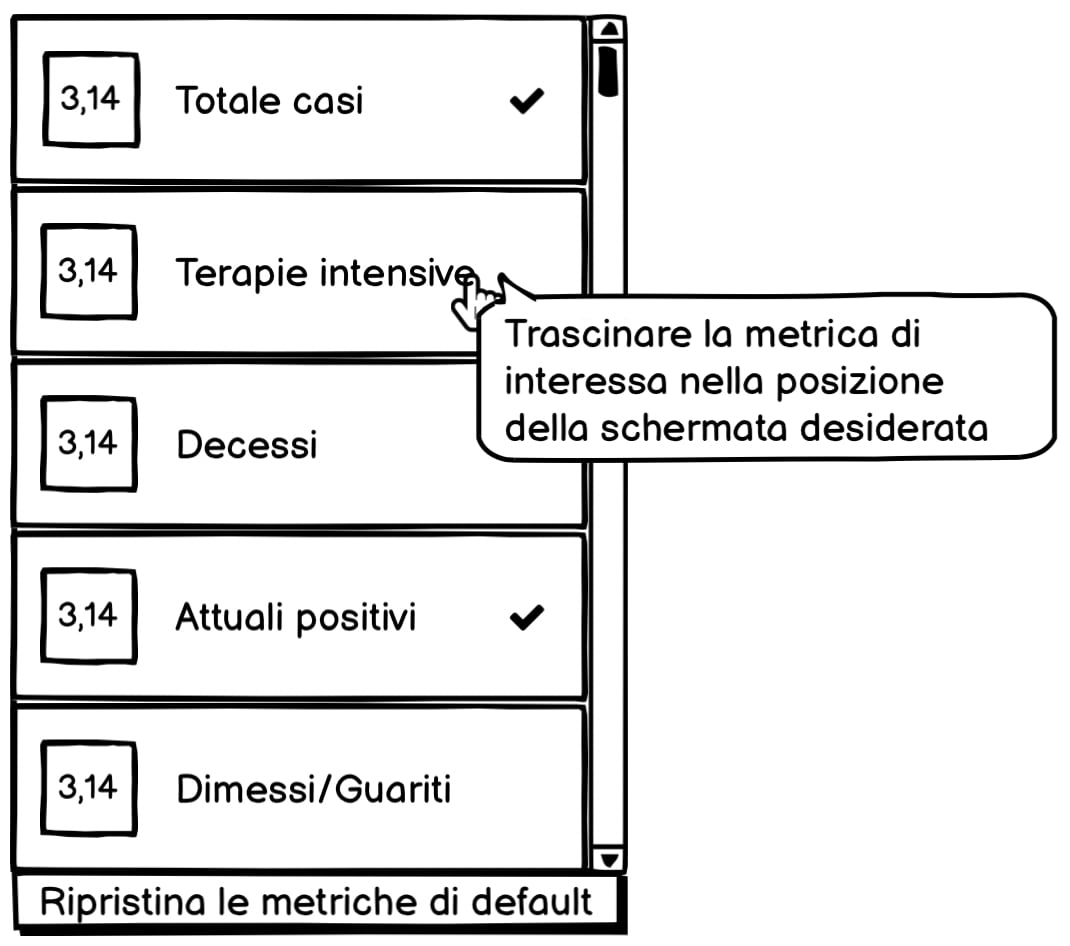
\includegraphics[width=0.5\textwidth]{wireframes/seleziona-metriche-tooltip}
        \caption{Tooltip in caso di click su un elemento della lista.}
        \label{fig:seleziona-metriche-tooltip}
    \end{subfigure}
    \caption{Seleziona metriche.}
\end{figure}


\paragraph{Seleziona data}\mbox{}\\
I widget per selezionare la data, apribili tramite il bottone tra le due frecce, sono di due tipi: quello mostrato in Figura \ref{fig:header-data-singola} permette di inserire un singolo giorno e l'altro mostrato in Figura \ref{fig:header-data-range} che permette d'inserire un range di date.\\

\begin{figure}[H]
    \begin{subfigure}[b]{0.5\textwidth}
        \centering
        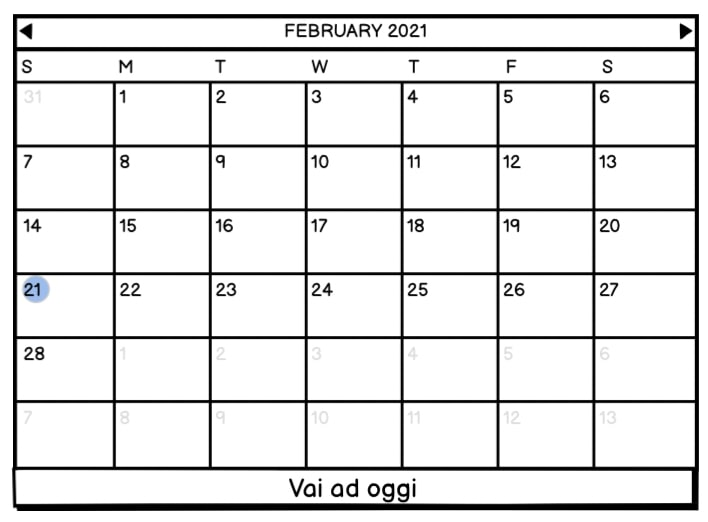
\includegraphics[width=0.77\textwidth]{wireframes/header-data-singola}
        \caption{Widget per selezionare una data singola.}
        \label{fig:header-data-singola}
    \end{subfigure}
\hfill
    \begin{subfigure}[b]{0.5\textwidth}
        \centering
        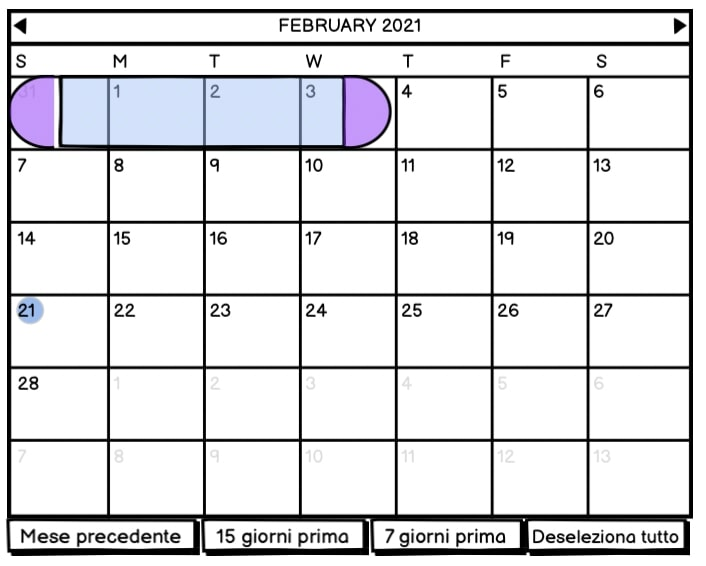
\includegraphics[width=0.7\textwidth]{wireframes/header-data-range}
        \caption{Widget per selezionare un range di date.}
        \label{fig:header-data-range}
    \end{subfigure}
    \caption{Widget per selezionare la data.}
\end{figure}
\noindent
Nel widget per selezionare una data singola (Figura \ref{fig:header-data-singola}) vi è bottone ``Vai ad oggi" per tornare rapidamente alla data odierna.\\
Nel widget per selezionare un range di date (Figura \ref{fig:header-data-range}) vi sono diversi bottoni che permettono agevolmente di andare al mese precedente, ai quindici giorni precedenti, ai sette giorni precedenti o di deselezionare il range.\\
In Figura \ref{fig:header-data-aperta}, è mostrato l'header e il widget calendario aperto.

\begin{figure}[H]
    \centering
    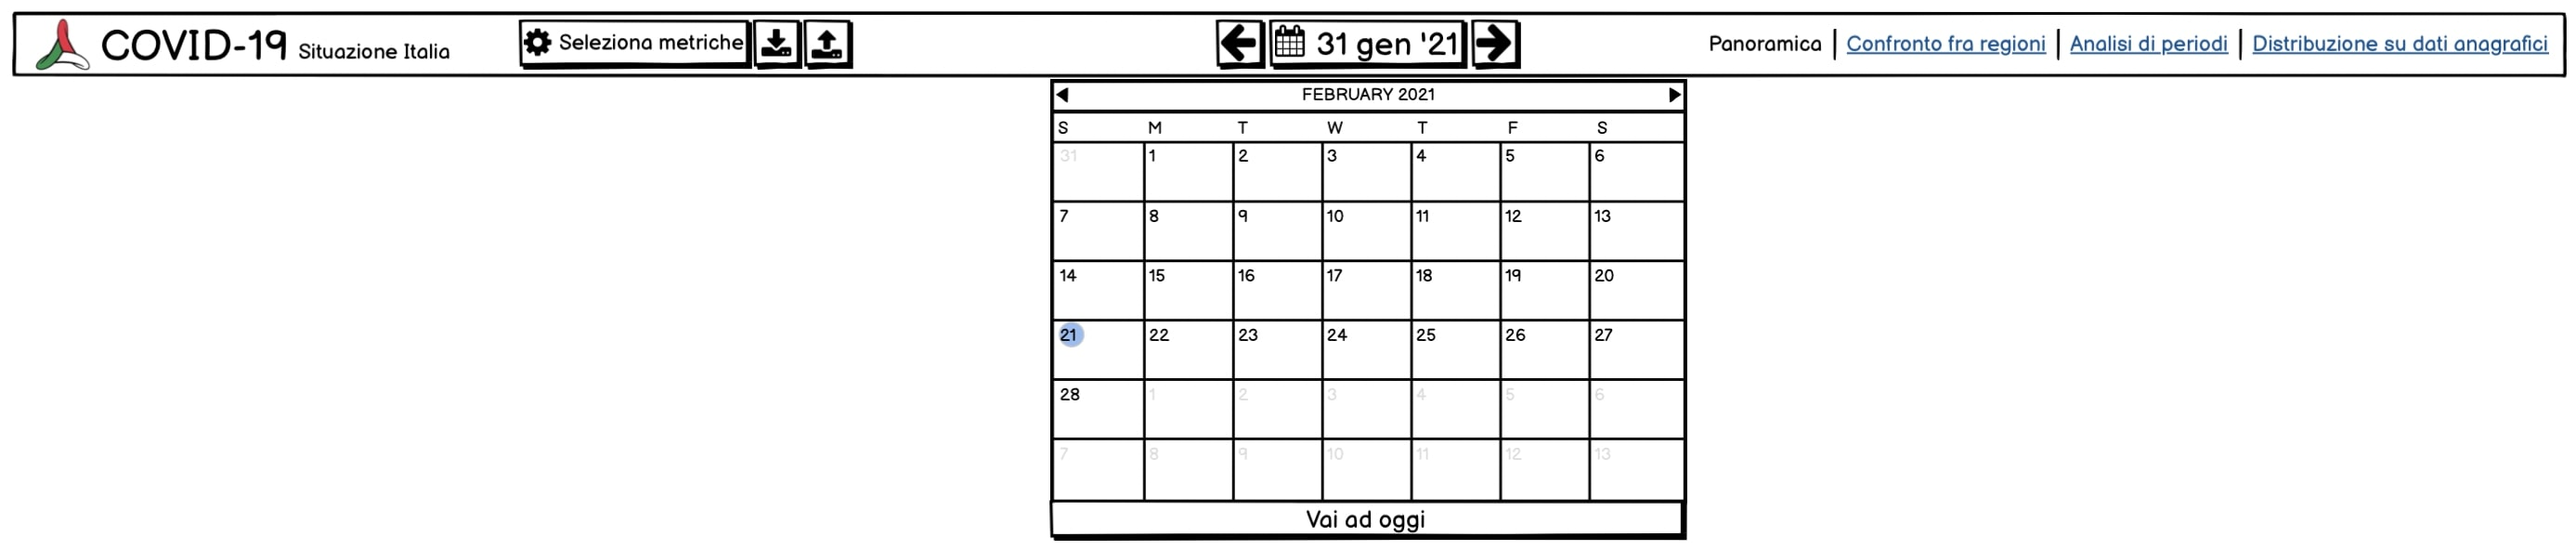
\includegraphics[width=1\columnwidth]{wireframes/header-data-aperta}
    \caption{Header con data aperta.}\label{fig:header-data-aperta}
\end{figure}

\begin{bclogo}{Iterazioni sul widget calendario}
    Inizialmente avevamo usato un semplice selettore di date (Figura \ref{fig:selettore-data-singola-vecchia}): solo in iterazioni successive, abbiamo arricchito l'interazione con bottoni di shortcut alla base del widget stesso.
\begin{figure}[H]
    \centering
    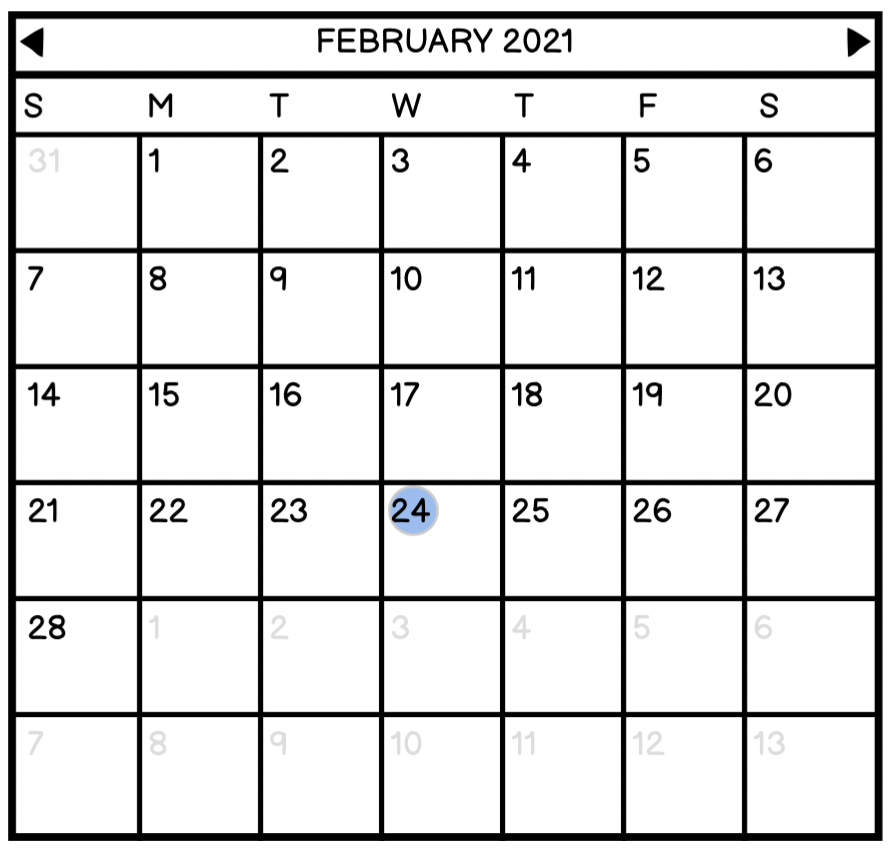
\includegraphics[width=0.3\columnwidth]{wireframes/selettore-data-singola-vecchia}
    \caption{Prima versione del selettore di date.}\label{fig:selettore-data-singola-vecchia}
\end{figure}
\end{bclogo}

\begin{figure}[H]
    \centering
    
\includegraphics[width=1\columnwidth]{wireframes/footer}
    \caption{Footer comune a tutte le schermate}
    \label{fig:footer}
\end{figure}

\paragraph{Footer}\mbox{}\\
Nel footer (Figura \ref{fig:footer}) vi sono alcune informazioni, quali link per le pagine istituzionali e le fonti dai quali i dati sono stati recuperati; a partire da destra, compaiono:
\begin{itemize}
    \item logo della Repubblica Italiana;
    \item logo e nome della DPC;
    \item link alle fonti e data dell'ultimo aggiornamento;
    \item link ai siti istituzionali.
\end{itemize}

\begin{bclogo}{Iterazioni sul footer}
    Le prime versioni del footer erano sprovviste della data dell'ultimo aggiornamento, tuttavia ci siamo resi conto che tale informazione era essenziale per i giornalisti, i quali hanno necessità di conoscere l'ultimo aggiornamento dei dati che stanno riportando nei loro articoli.
\begin{figure}[H]
    \centering
    
\includegraphics[width=1\columnwidth]{wireframes/footer-vecchio}
    \caption{Prima versione del footer.}
    \label{fig:footer-vecchio}
\end{figure}
\end{bclogo}


\subsubsection{Panoramica}\label{ss:panoramica}
\begin{figure}[H]
    \centering
    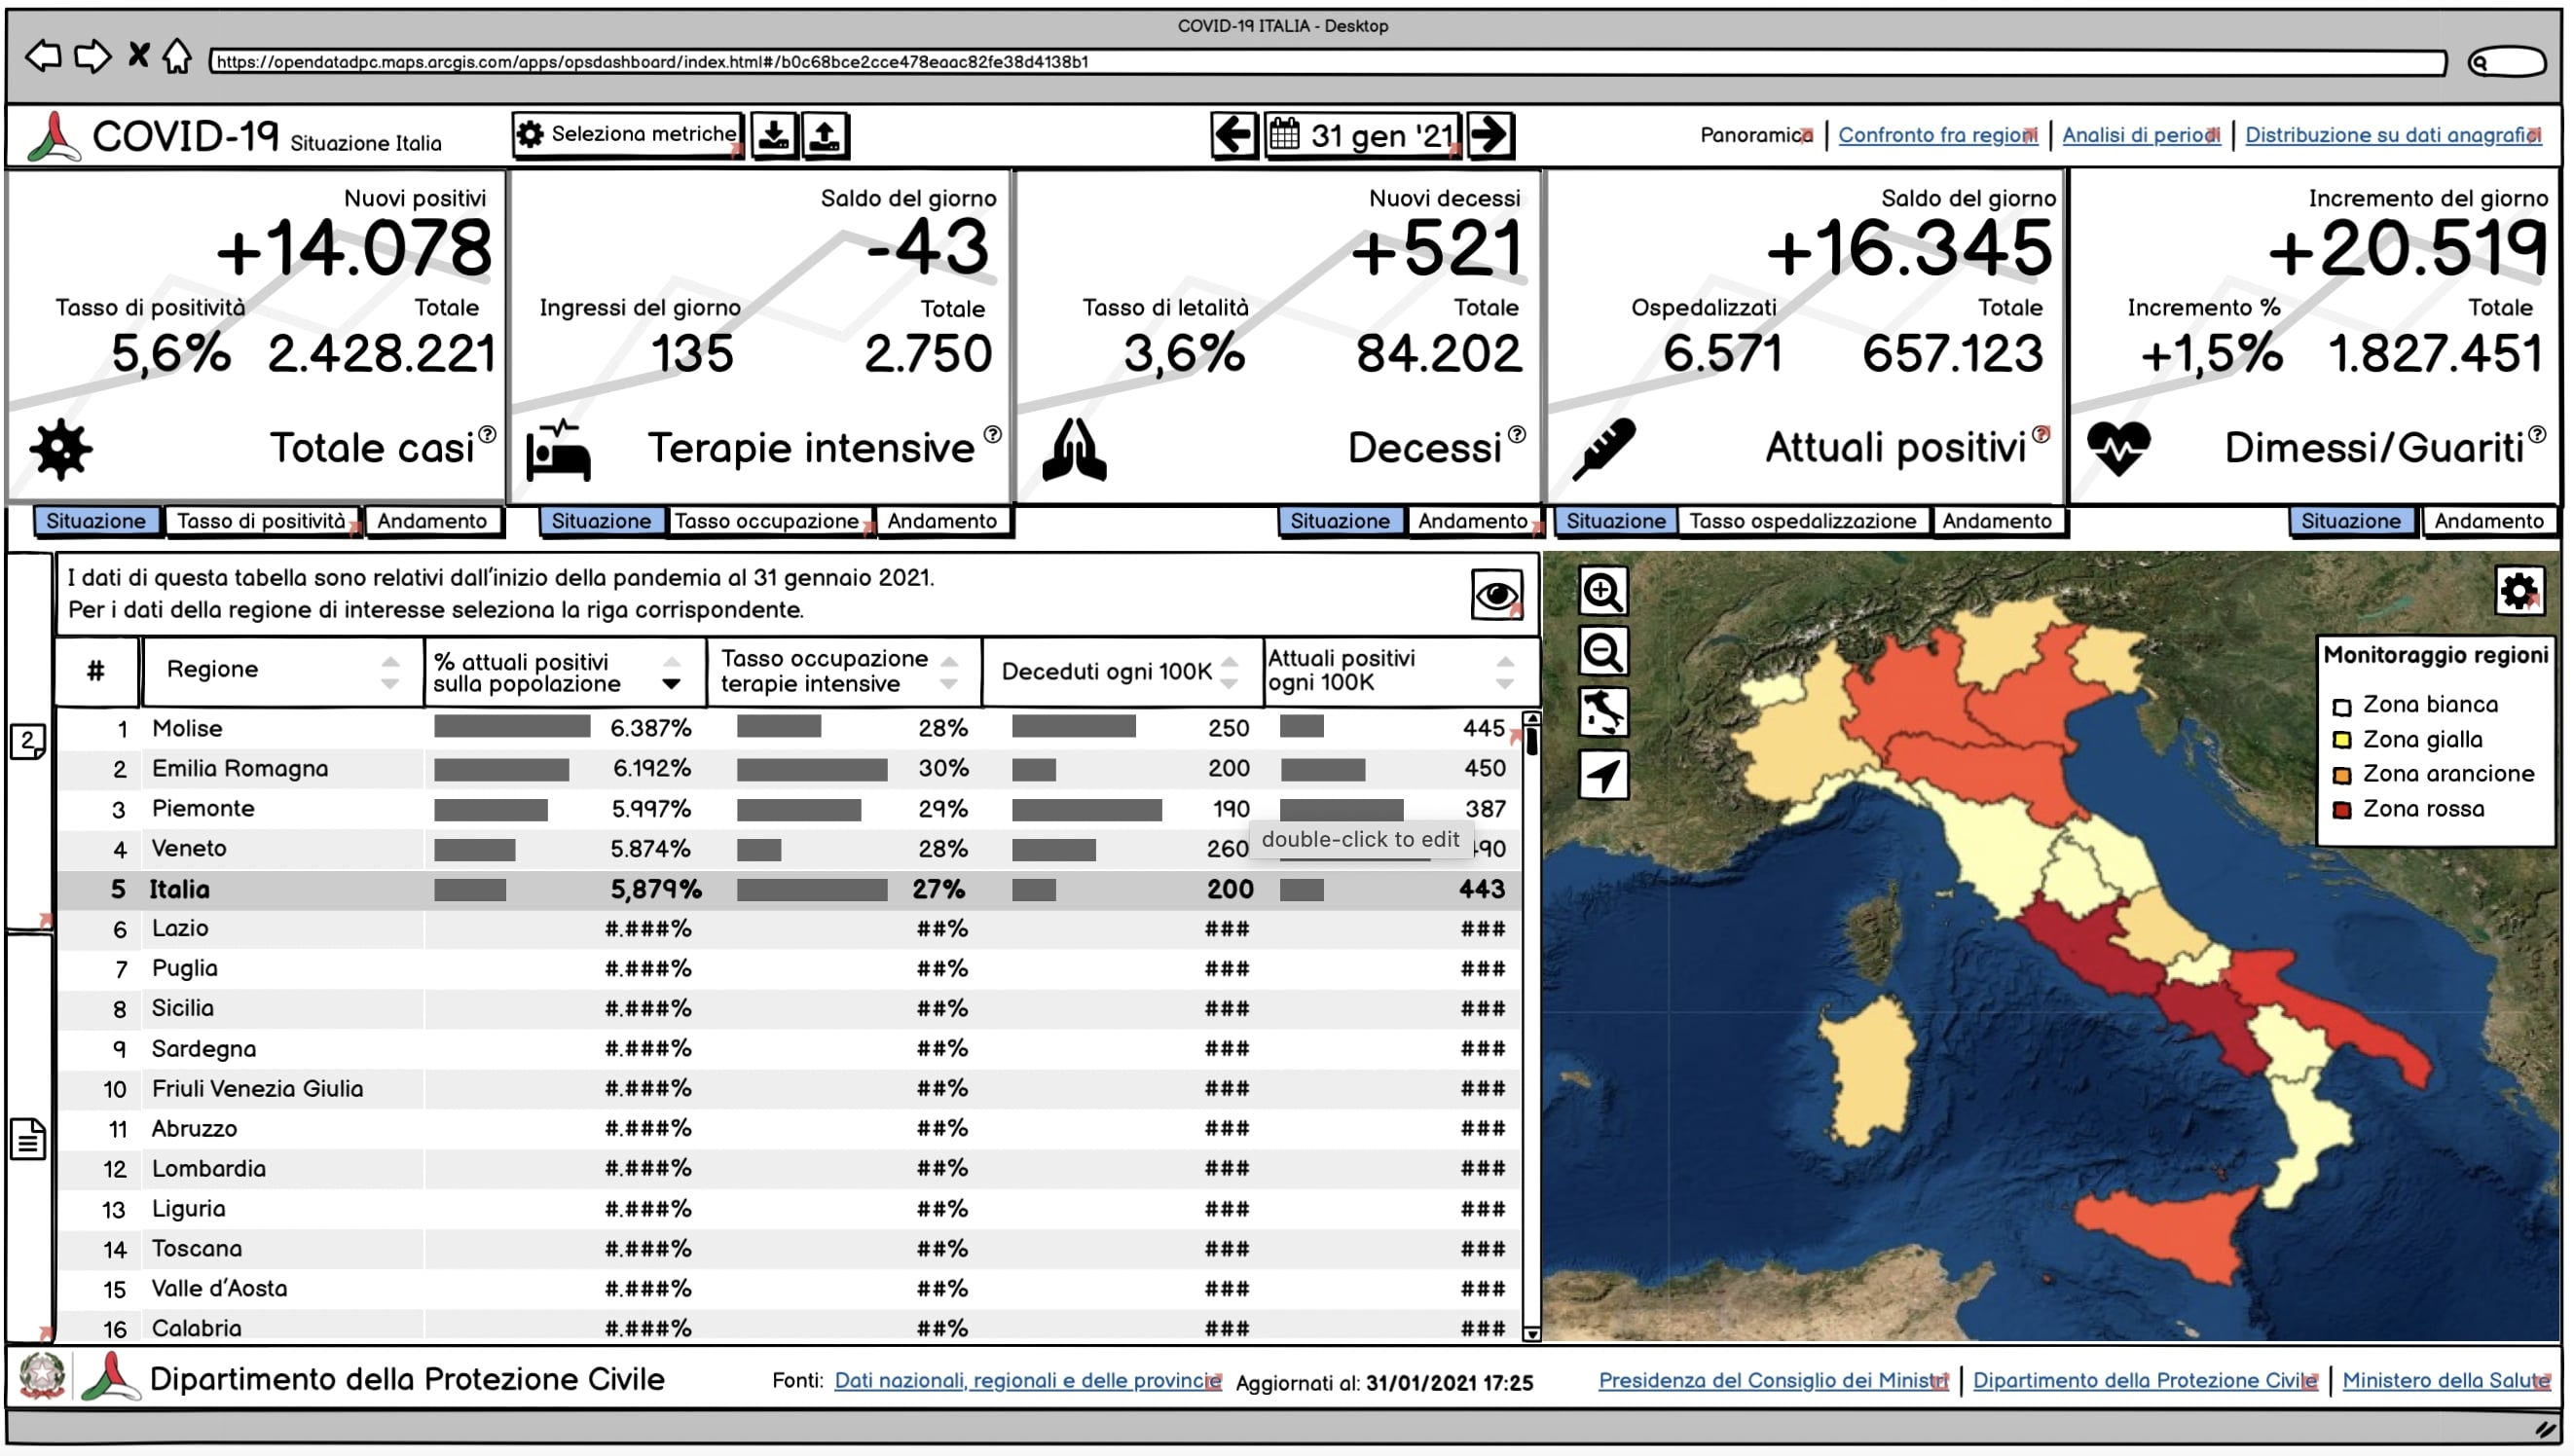
\includegraphics[width=1\columnwidth]{wireframes/panoramica}
    \caption{Schermata ``Panoramica''}
    \label{fig:panoramica}
\end{figure}
La schermata ``Panoramica'' è la prima schermata che un utente incontra aprendo la dashboard.\\
\`E possibile dividere visivamente la schermata in due fasce: la fascia superiore che presenta cinque ``Box numerici'' e una fascia inferiore che presenta dei pulsanti per aprire le sidebar delle note e dei provvedimenti, una tabella e una \textit{heat map}.\\

\paragraph{Box numerici}\mbox{}\\
\begin{figure}[H]
    \centering
    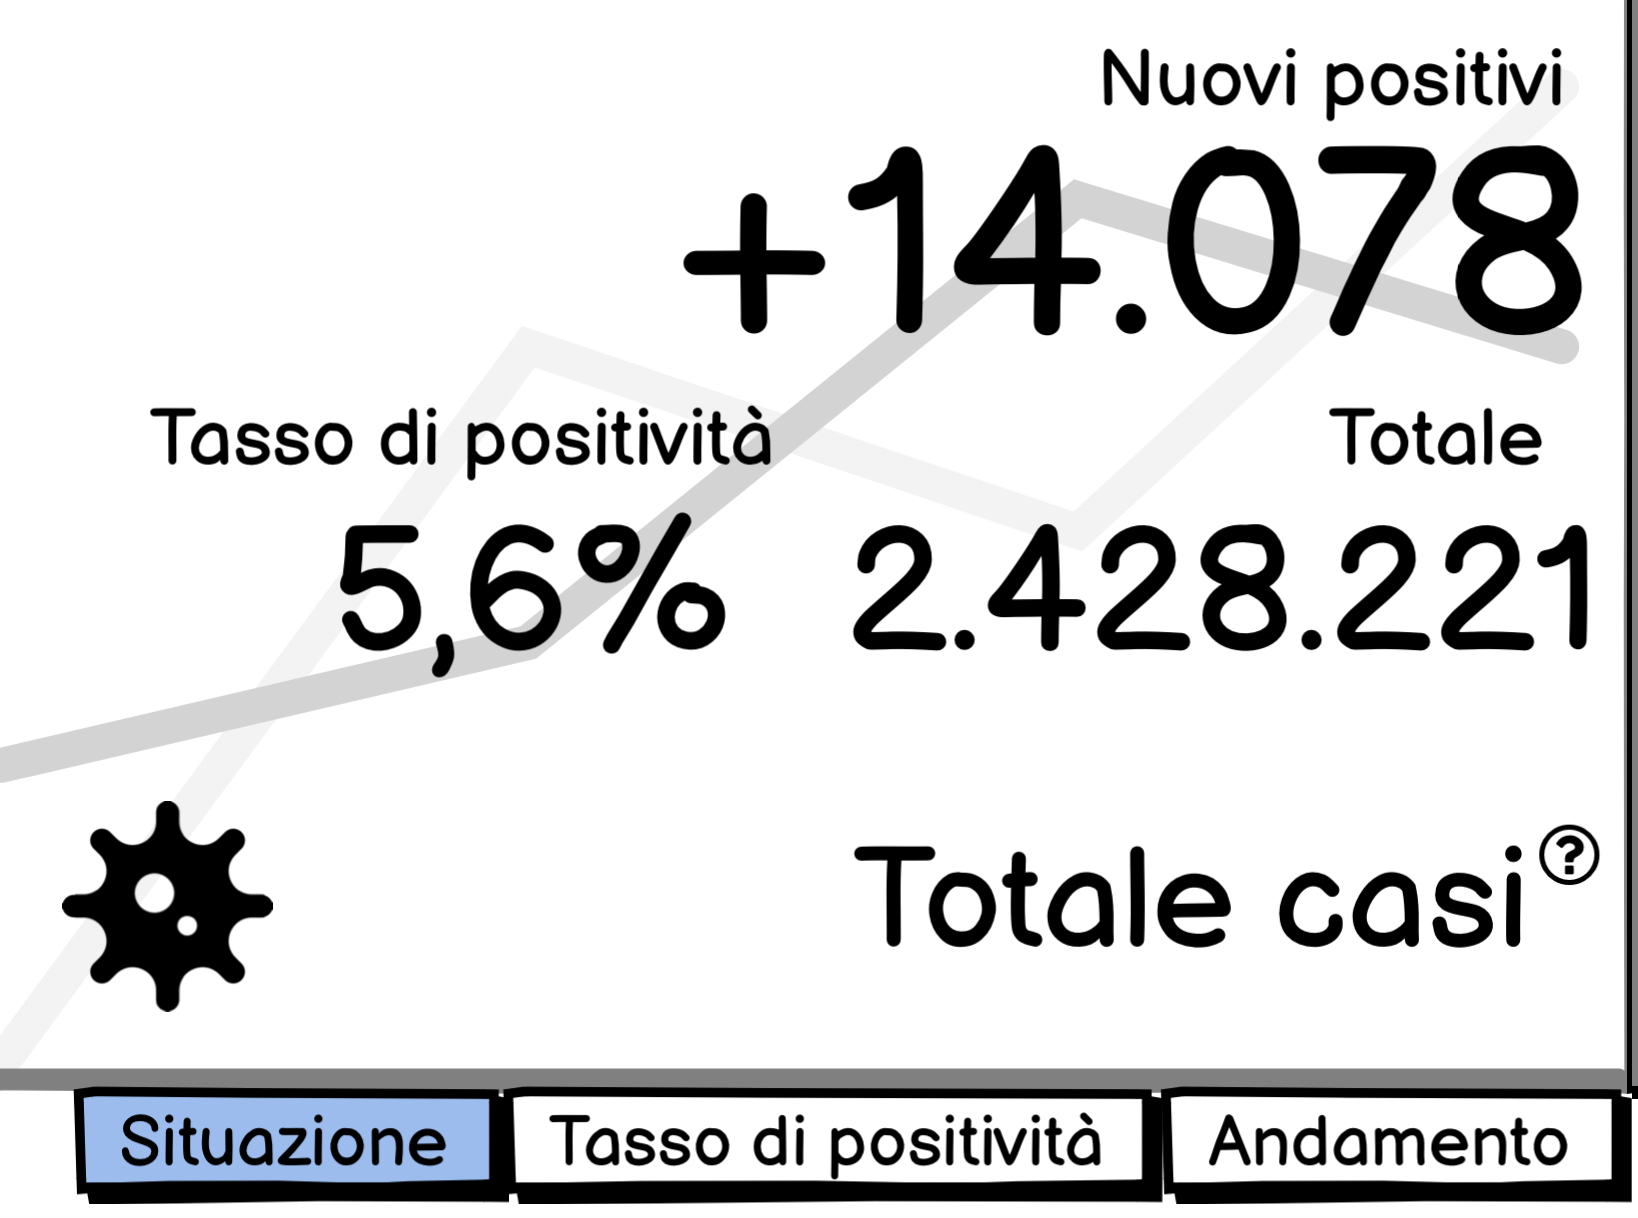
\includegraphics[width=0.5\columnwidth]{wireframes/box-numerico}
    \caption{Esempio di box numerico.}
    \label{fig:box-numerico}
\end{figure}
\noindent
I cinque box numerici, di cui Figura \ref{fig:box-numerico} ne è un esempio, sono composti dal nome della metrica, posto in basso e avente la dimensione del font maggiore, e tre valori numerici, ognuno dei quali è preceduto da un'etichetta che esplicita a cosa si riferisce.\\
In ogni box, è presente, in basso a sinistra, un'icona che aiuta il giornalista nell'individuare la metrica trattata e a ridurne il carico il carico cognitivo. Come sfondo del box vi è la curva che rappresenta l'andamento della metrica.\\
Al di sotto di ogni box numerico vi sono dei pulsanti che cambiano il contenuto del box numerico: al netto di bottoni auto-esplicativi, il pulsante ``Andamento'' mostra un grafico con l'andamento della metrica (Figura \ref{fig:box-andamento}), il pulsante ``Tasso di \dots'' mostra una \textit{gauge} (Figura \ref{fig:box-gauge}) mentre il pulsante ``Situazione'' mostra il box numerico mostrato di default all'apertura della pagina.

\begin{figure}[H]
    \begin{subfigure}[b]{0.5\textwidth}
        \centering
        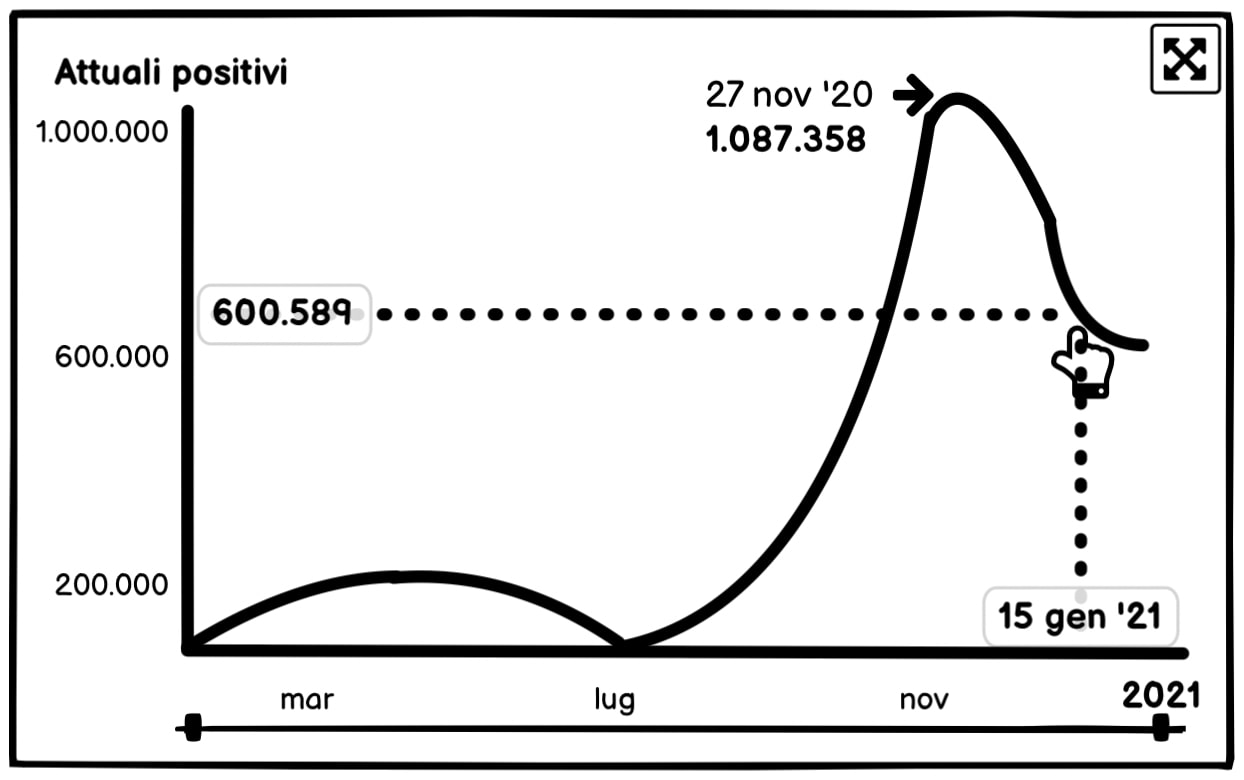
\includegraphics[width=1\textwidth]{wireframes/box-andamento}
        \caption{Box con grafico dell'andamento.}
        \label{fig:box-andamento}
    \end{subfigure}
\hfill
    \begin{subfigure}[b]{0.51\textwidth}
        \centering
        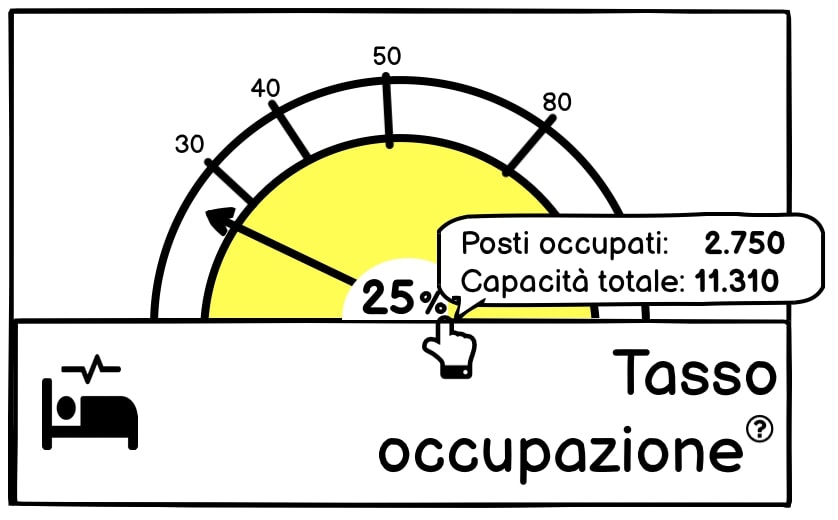
\includegraphics[width=1\textwidth]{wireframes/box-gauge}
        \caption{Box con gauge.}
        \label{fig:box-gauge}
    \end{subfigure}
    \caption{Viste alternative del ``Box numerico'' nella schermata ``Panoramica''.}
\end{figure}

\begin{bclogo}{Iterazioni sui box numerici}
    I box numerici hanno subito diverse modifiche prima di arrivare alla versione finale. Siamo partiti con l'idea di dover mostrare la variazione, il totale raggiunto e un icona (Figura \ref{fig:box-numerici-prima-versione}).
\begin{figure}[H]
    \begin{subfigure}[b]{0.5\textwidth}
        \centering
        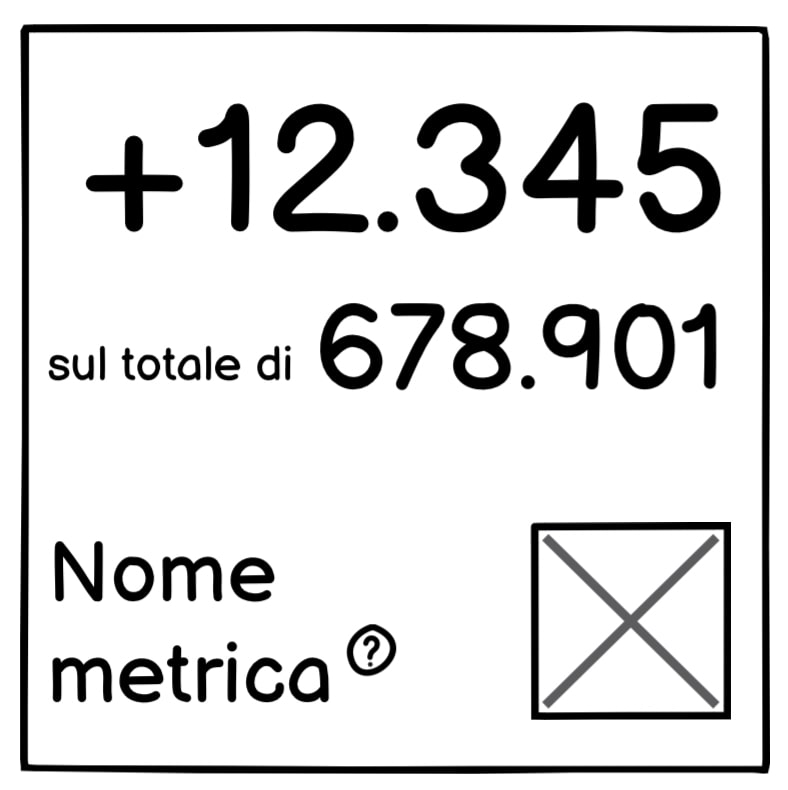
\includegraphics[width=.5\textwidth]{wireframes/box-numerici-prima-versione}
        \caption{Prima alternativa della prima versione dei box numerici.}
        \label{fig:box-numerici-prima-versione1}
    \end{subfigure}
    \begin{subfigure}[b]{0.5\textwidth}
        \centering
        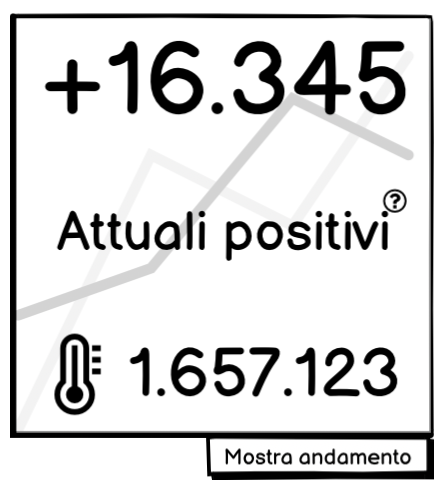
\includegraphics[width=.5\textwidth]{wireframes/box-numerici-prima-versione-2}
        \caption{Seconda alternativa della prima versione dei box numerici.}
        \label{fig:box-numerici-prima-versione2}
    \end{subfigure}
    \caption{Prime versione dei box numerici}
    \label{fig:box-numerici-prima-versione}
\end{figure}
\noindent
Dopo aver scelto di proseguire lo sviluppo del design di Figura \ref{fig:box-numerici-prima-versione1}, abbiamo riorganizzato i componenti all'interno del box ottenendo quando mostrato in Figura \ref{fig:box-numerici-seconda-versione}.

\begin{figure}[H]
    \centering
    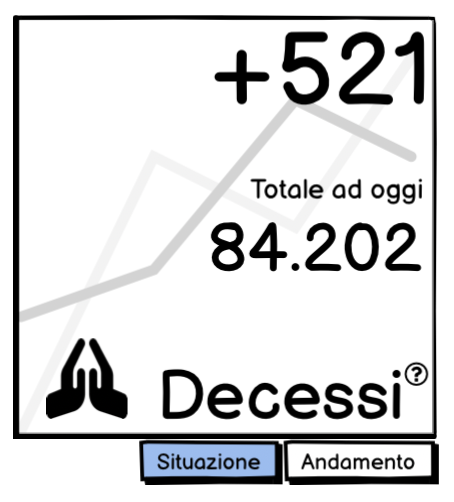
\includegraphics[width=0.3\columnwidth]{wireframes/box-numerici-seconda-versione}
    \caption{Seconda versione dei box numerici.}
    \label{fig:box-numerici-seconda-versione}
\end{figure}
\noindent
Infine, rendendoci conto che avevamo ancora spazio a disposizione abbiamo aggiunto un ulteriore valore, quale un valore percentuale, ottenendo così il design finale.
\end{bclogo}
\clearpage
\paragraph{Box con andamento}\mbox{}\\
I box con andamento possono avere due tipi di grafico in base alla metrica di cui si vuole osservare l'andamento: uno con una curva monotona crescente, per le metriche cumulate (Figura \ref{fig:box-andamento-monotono}) e un altro con una curva che non presenta monotonia (Figura \ref{fig:box-andamento-no-monotonia}). 
\begin{figure}[H]
    \begin{subfigure}[b]{0.5\textwidth}
        \centering
        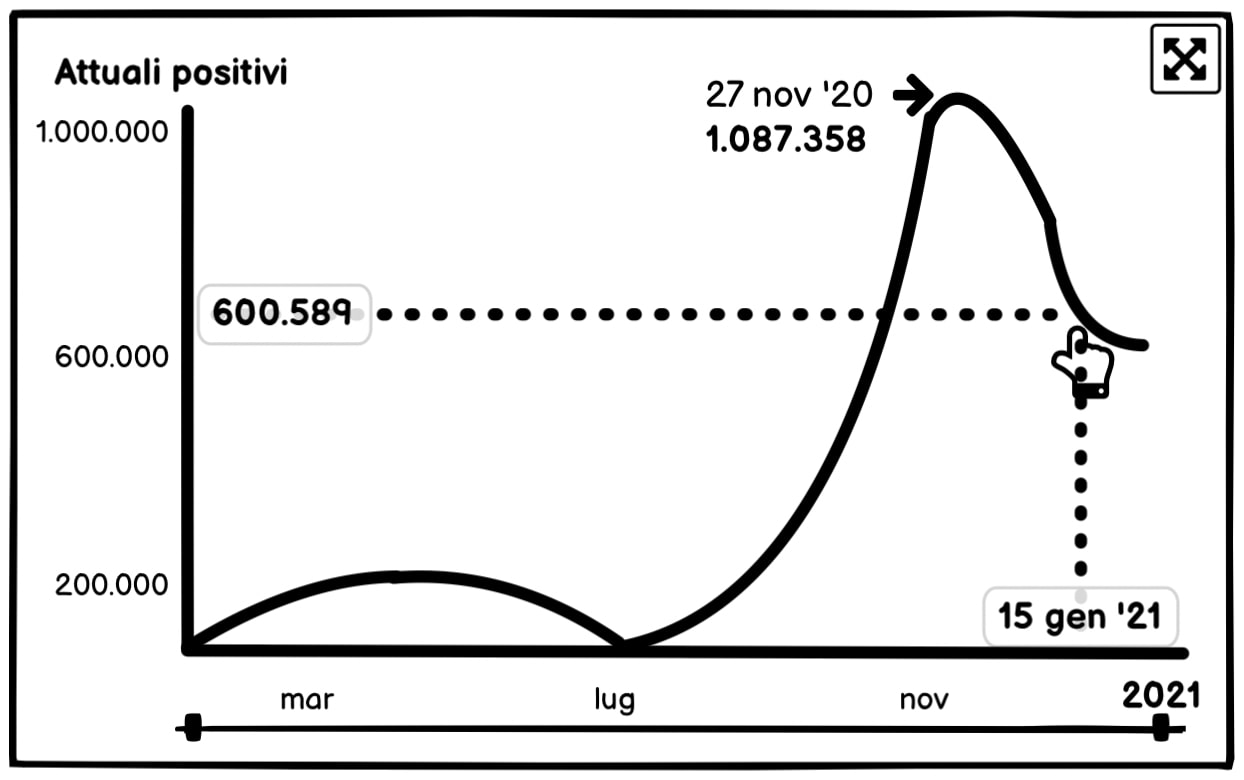
\includegraphics[width=1\textwidth]{wireframes/box-andamento}
        \caption{Box con grafico dell'andamento con una curva che non presenta monotonia.}\label{fig:box-andamento-no-monotonia}
    \end{subfigure}
\hfill
    \begin{subfigure}[b]{0.5\textwidth}
        \centering
        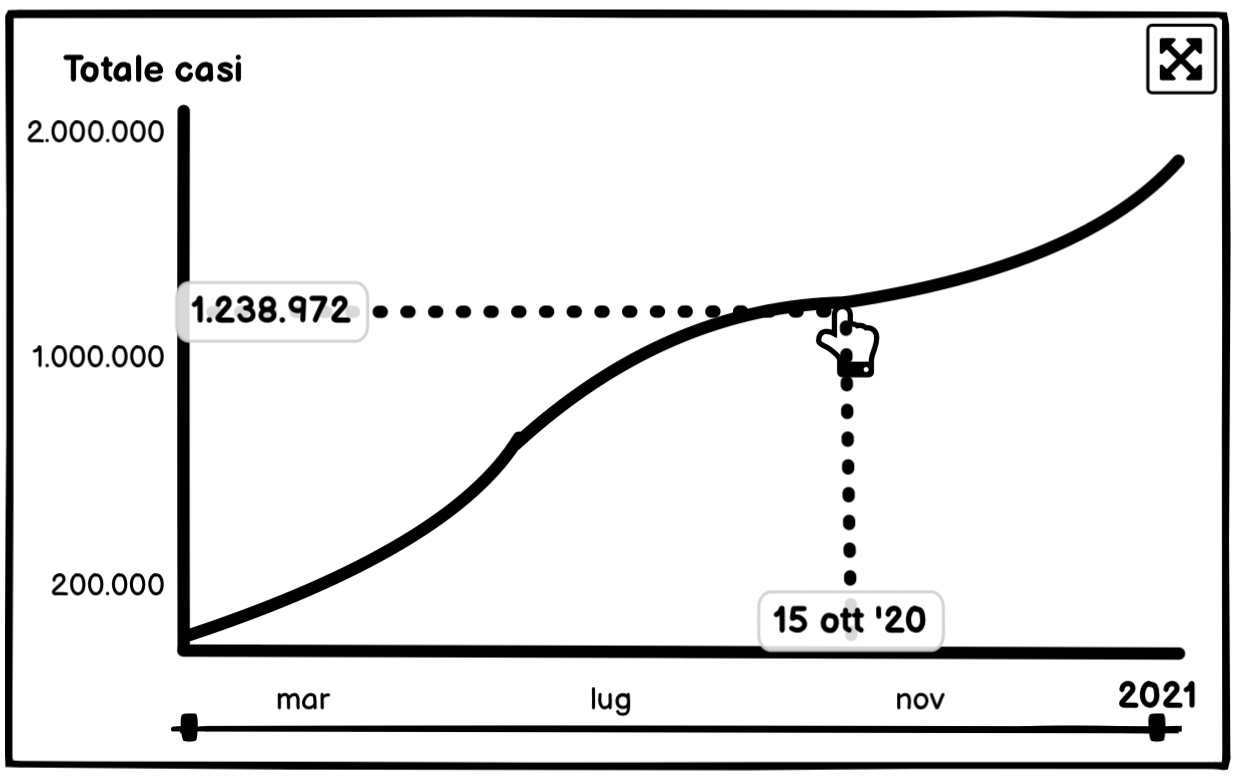
\includegraphics[width=1\textwidth]{wireframes/box-andamento-monotono}
        \caption{Box con grafico dell'andamento con una curva monotona crescente.}
        \label{fig:box-andamento-monotono}
    \end{subfigure}
    \caption{Differenti tipi di grafico dell'andamento di una metrica.}
\end{figure}
\noindent
In Figura \ref{fig:box-andamento-no-monotonia} è presente un indicatore al valore massimo raggiunto, che, a differenza, in Figura \ref{fig:box-andamento-monotono} non è presente.\\
In comune a entrambi in grafici vi è uno slider sotto l'asse delle $x$ con due selettori, muovendo i quali si può modificare la data di inizio e di fine della finestra temporale d'interesse.\\
Inoltre in caso si passi sopra al grafico con il cursore, compare un tooltip che indica i valori raggiunti il giorno indicato dalla proiezione sull'asse delle $x$.\\
In questi grafici è presente un pulsante in alto a destra che permette di visualizzare il grafico a schermo intero, come mostrato in Figura \ref{fig:grafico-full-screen}. Lo stesso pulsante può essere utilizzato per far tornare il grafico alla sua dimensione originaria.
\begin{figure}[H]
    \centering
    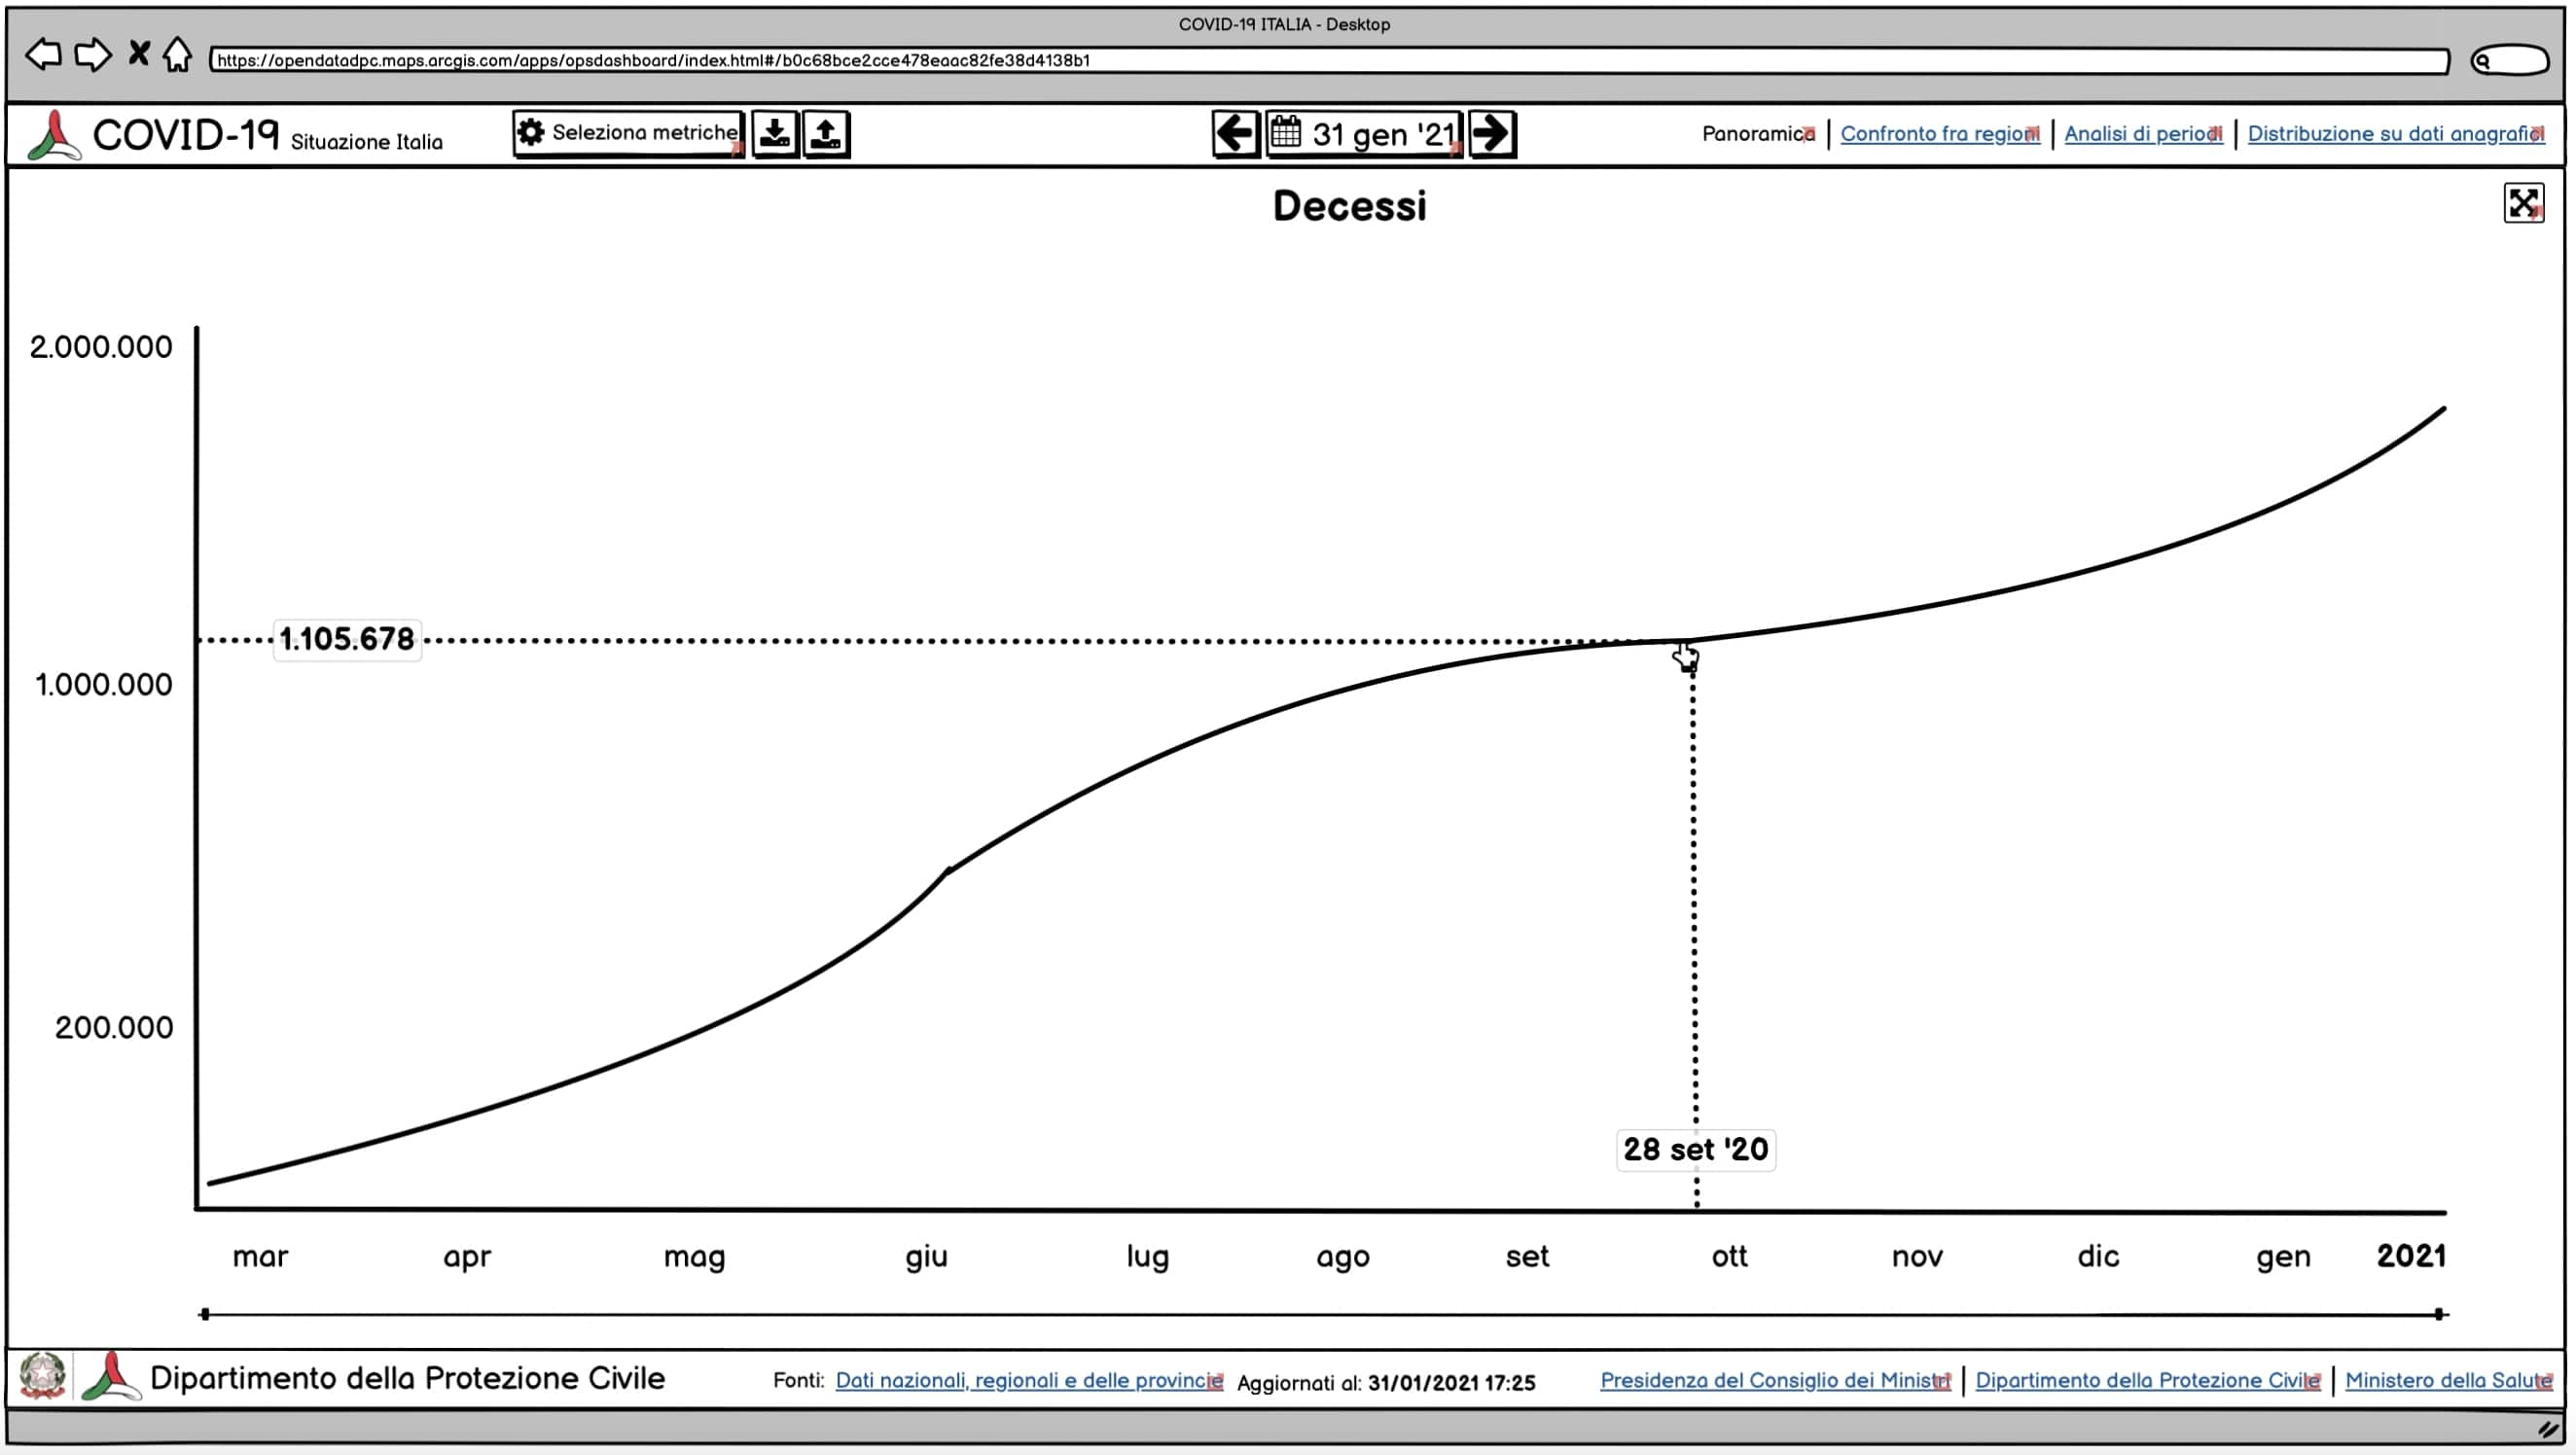
\includegraphics[width=0.6\columnwidth]{wireframes/grafico-full-screen}
    \caption{Grafico a schermo intero.}
    \label{fig:grafico-full-screen}
\end{figure}

\paragraph{Box con gauge}\mbox{}\\
I box con gauge sono utili per contestualizzare una certa metrica (tasso di positività, tasso di occupazione delle terapie intensive). In caso vi si passi sopra col cursore, compare un tooltip che mostra i valori assoluti di quella metrica (Figura \ref{fig:box-gauge}).

\begin{bclogo}{Iterazioni sui box con gauge}
    Inizialmente avevamo pensato a due possibili tipi di gauge, mostrati in Figura \ref{fig:opzioni-gauge}; abbiamo optato per l'opzione mostrata da Figura \ref{fig:opzione-gauge-finale} in quanto ci piaceva maggiormente e ci permetteva di occupare meglio gli spazi.

    \begin{figure}[H]
    \begin{subfigure}[b]{0.5\textwidth}
        \centering
        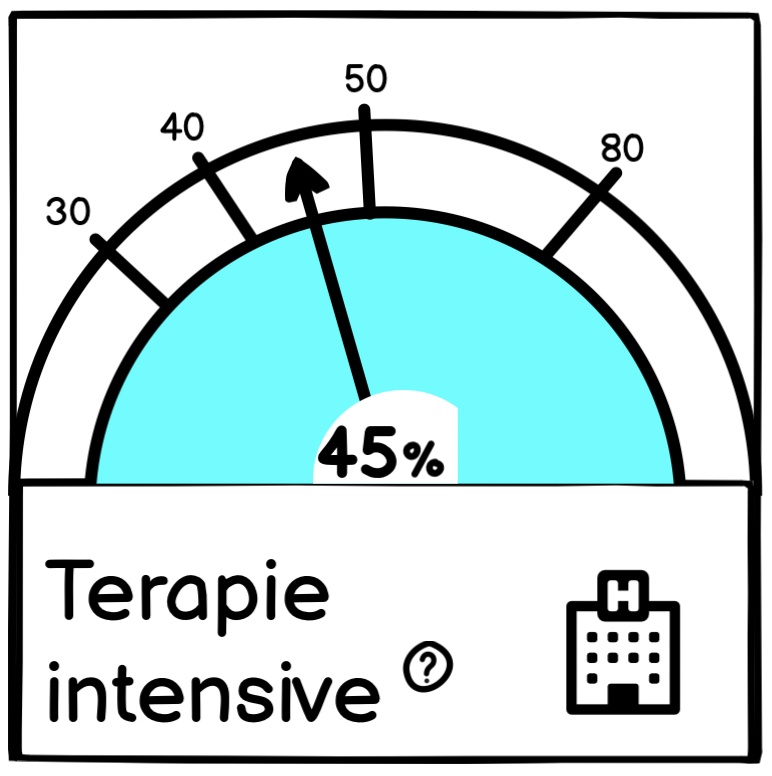
\includegraphics[width=0.7\textwidth]{wireframes/box-con-gauge-scelta}
        \caption{Design finale di un box con gauge.}
        \label{fig:opzione-gauge-finale}
    \end{subfigure}
\hfill
    \begin{subfigure}[b]{0.5\textwidth}
        \centering
        
\includegraphics[width=0.7\textwidth]{wireframes/opzione-gauge-scartata}
        \caption{Design scartata di un box con gauge.}
        \label{fig:opzione-gauge-scartata}
    \end{subfigure}
    \caption{Differenti tipi di box con gauge.}
    \label{fig:opzioni-gauge}
\end{figure}

\end{bclogo}

\clearpage
\paragraph{Box con areogramma}\mbox{}\\
I box con areogramma sono stati usati per mostrare come in numeri di una metrica si distribuiscono in percentuale. Un esempio è quello usato per mostrare come si differenziano i ricoveri tra le persone ricoverate con sintomi e le persone ricoverate in terapia intensiva.
\begin{figure}[H]
    \centering
    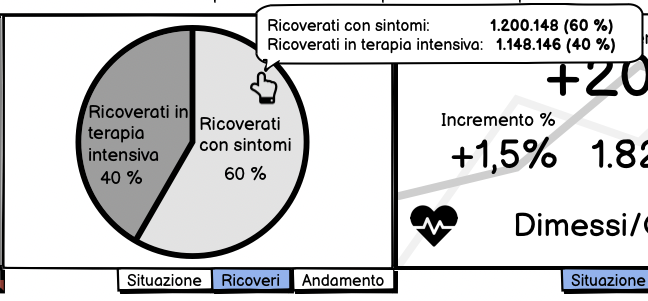
\includegraphics[width=0.5\columnwidth]{wireframes/box-con-areogramma}
    \caption{Esempio di box con areogramma.}\label{fig:box-areogramma}
\end{figure}

\clearpage
\paragraph{Sidebar delle note e dei provvedimenti}\mbox{}\\
Sulla destra, vi sono due pulsanti che al click aprono due sidebar: una che mostra le note (Figura \ref{fig:note}), ordinate cronologicamente e, l'altro, che mostra i provvedimenti (Figura \ref{fig:provvedimenti}), anch'essi ordinati cronologicamente. 
\begin{figure}[H]
    \begin{subfigure}[b]{0.5\textwidth}
        \centering
        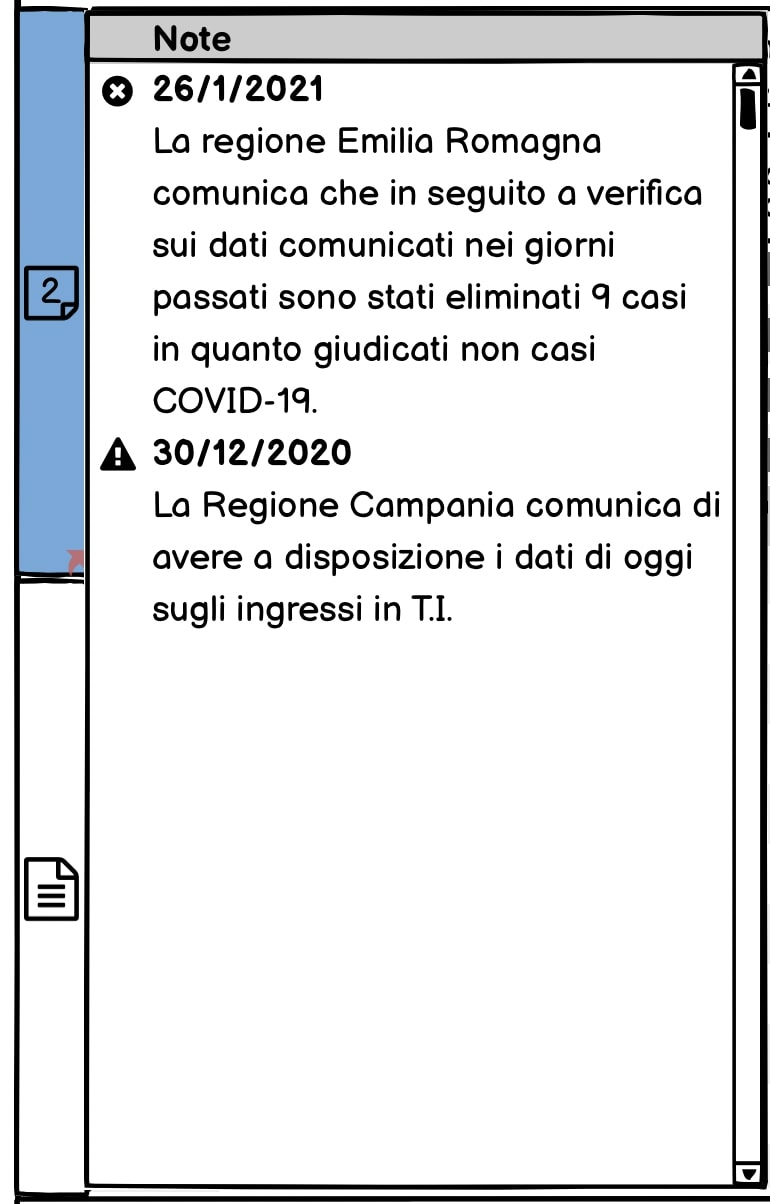
\includegraphics[width=1\textwidth]{wireframes/note}
        \caption{Sidebar delle note.}
        \label{fig:note}
    \end{subfigure}
\hfill
    \begin{subfigure}[b]{0.5\textwidth}
        \centering
        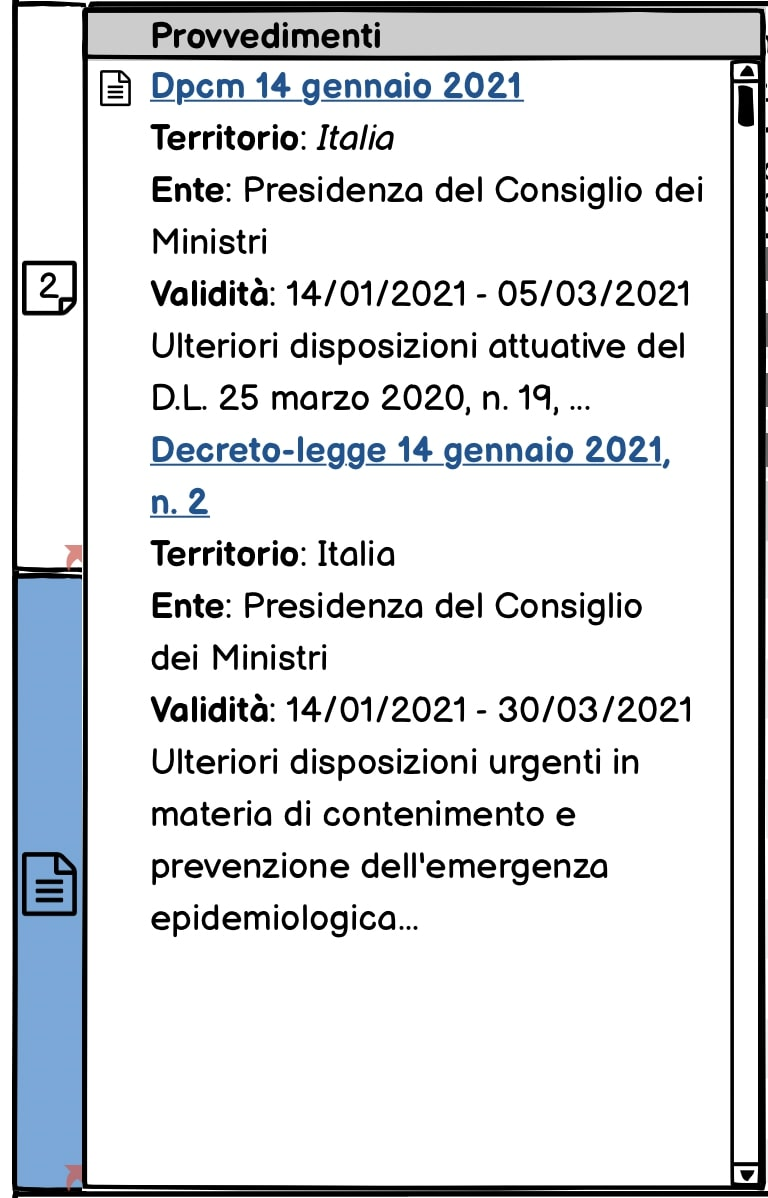
\includegraphics[width=1\textwidth]{wireframes/provvedimenti}
        \caption{Sidebar dei provvedimenti.}
        \label{fig:provvedimenti}
    \end{subfigure}
    \caption{Differenti tipi di grafico dell'andamento di una metrica.}
\end{figure}
\noindent
In caso venga pubblicata una nuova nota o un nuovo provvedimento mentre si sta utilizzando la dashboard, l'utente viene notificato con la comparsa del numero di nuove note o nuovi provvedimenti sul pulsante; nel caso di Figura \ref{fig:note} abbiamo simulato la presenza di due nuove note.

\clearpage
\paragraph{Tabella}\mbox{}\\
\begin{figure}[H]
    \centering
    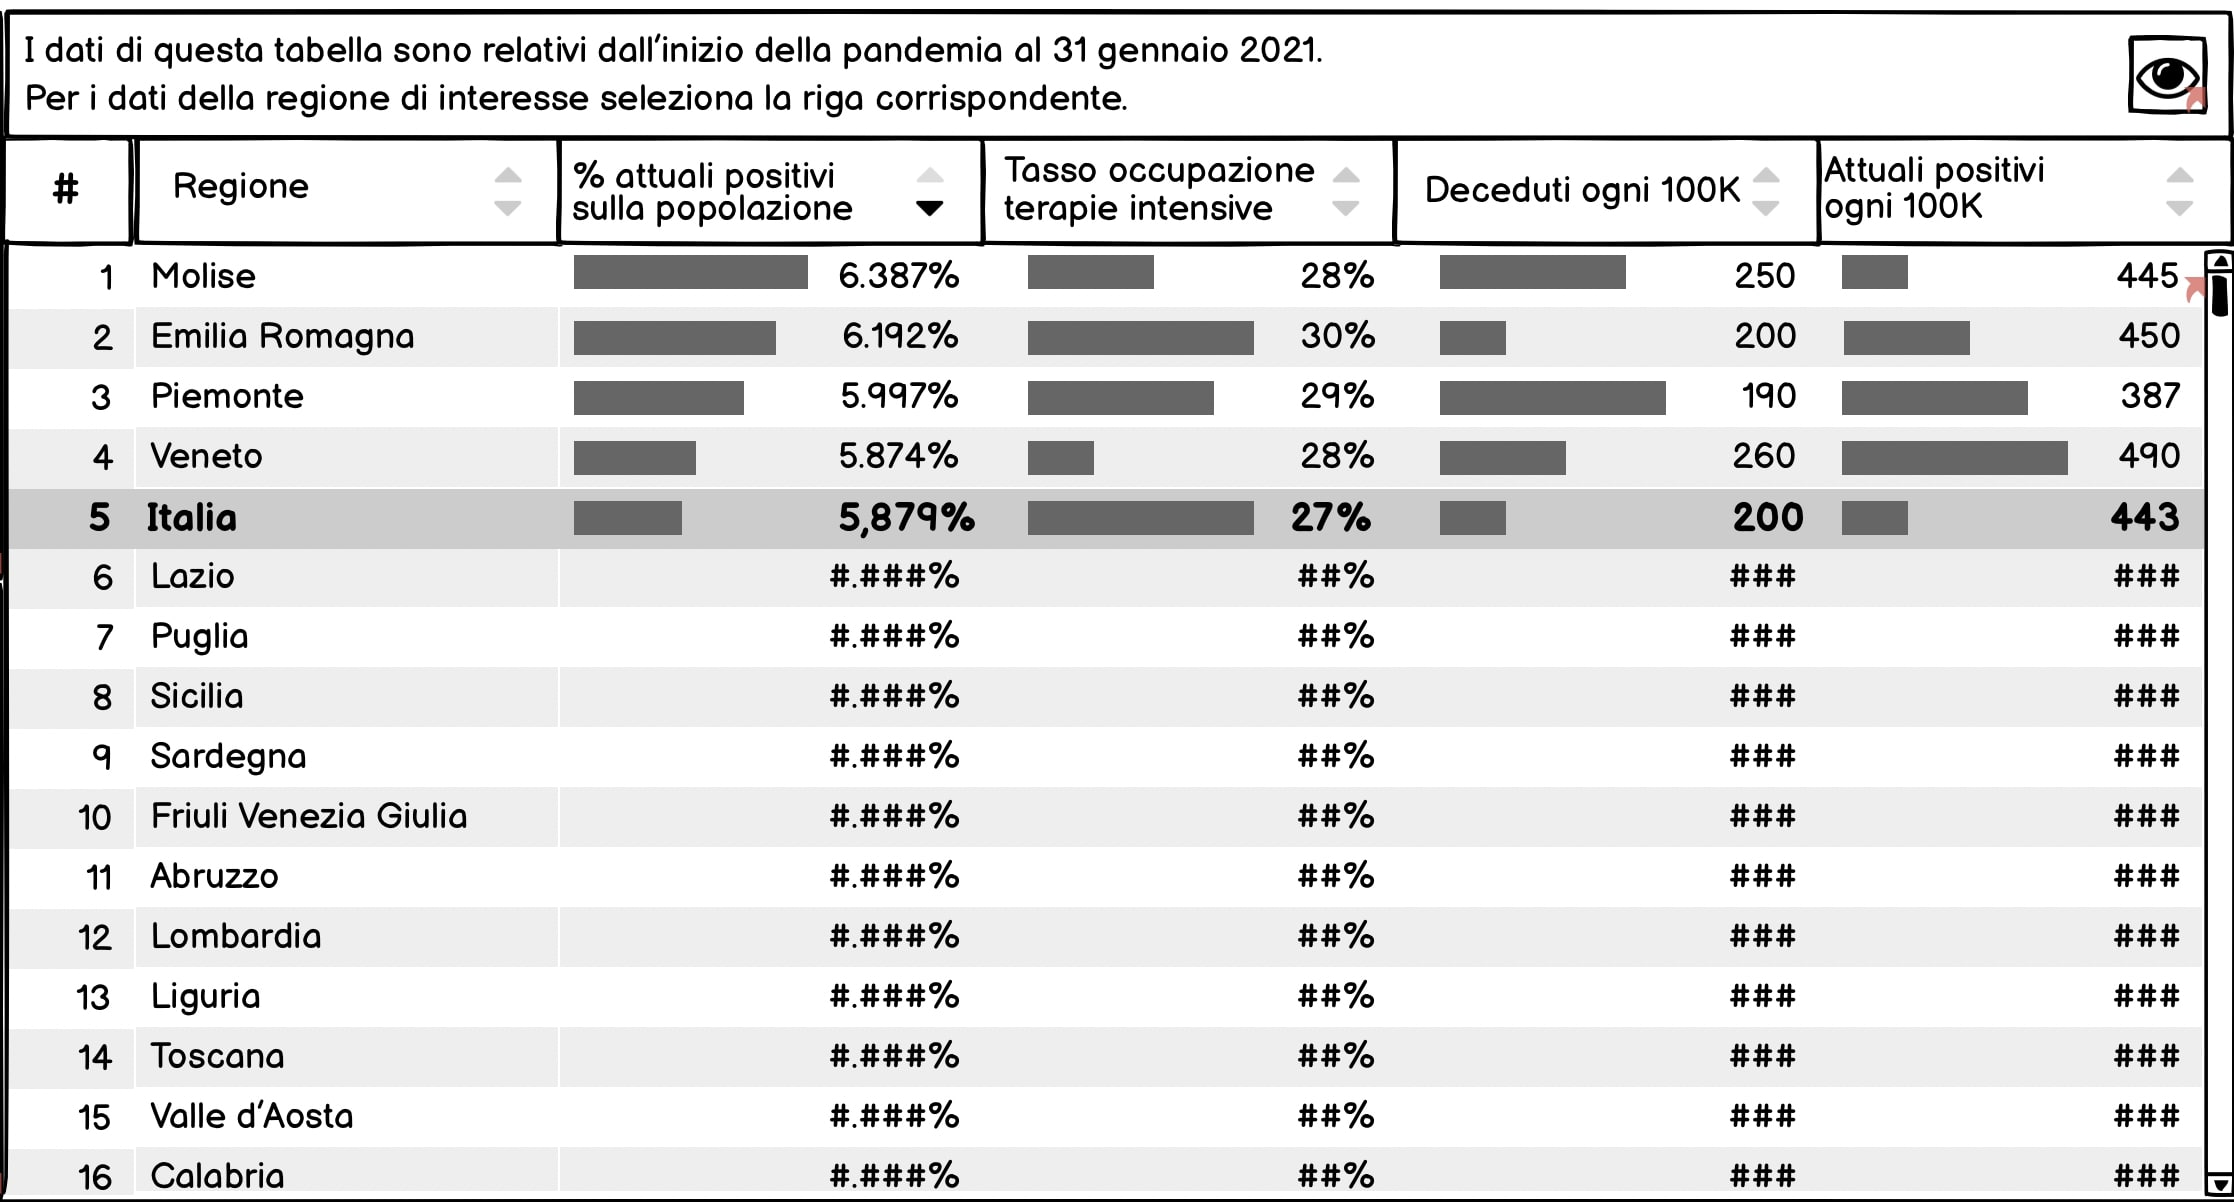
\includegraphics[width=0.7\columnwidth]{wireframes/tabella}
    \caption{Tabella delle regioni.}
    \label{fig:tabella}
\end{figure}
\noindent
Nella tabella in Figura \ref{fig:tabella} vi è l'elenco delle regioni italiane e i valori che hanno di certe metriche: queste possono essere modificate cliccando sul pulsante con icona a ghiera, cliccando sul quale si apre una lista di metriche come in Figura \ref{fig:lista-metriche-tabella} che possono essere selezionate tramite una \textit{check-box}.\\
Le colonne della tabella offrono la funzionalità di ordinamento per semplificare il confronto tra le diverse regioni, inoltre è presente una riga rappresentante la situazione dell'Italia in modo da permettere il confronto tra una regione e la media nazionale. In ogni cella i valori delle metriche sono affiancati a una barra che permette di confrontare più velocemente le diverse righe.\\
Cliccando su una regione i dati dell'intera schermata vengono aggiornati con i dati relativi a essa: a mo' d'esempio, cliccando sulla regione Molise si ottiene la schermata in Figura \ref{fig:panoramica-regione}. Nella tabella di questa vista sono presenti i dati relativi alle province della regione selezionata, alla regione stessa e alla nazione. Per tornare alla vista nazionale è possibile cliccare sulla riga dell'Italia nella tabella.
\begin{figure}[H]
    \centering
    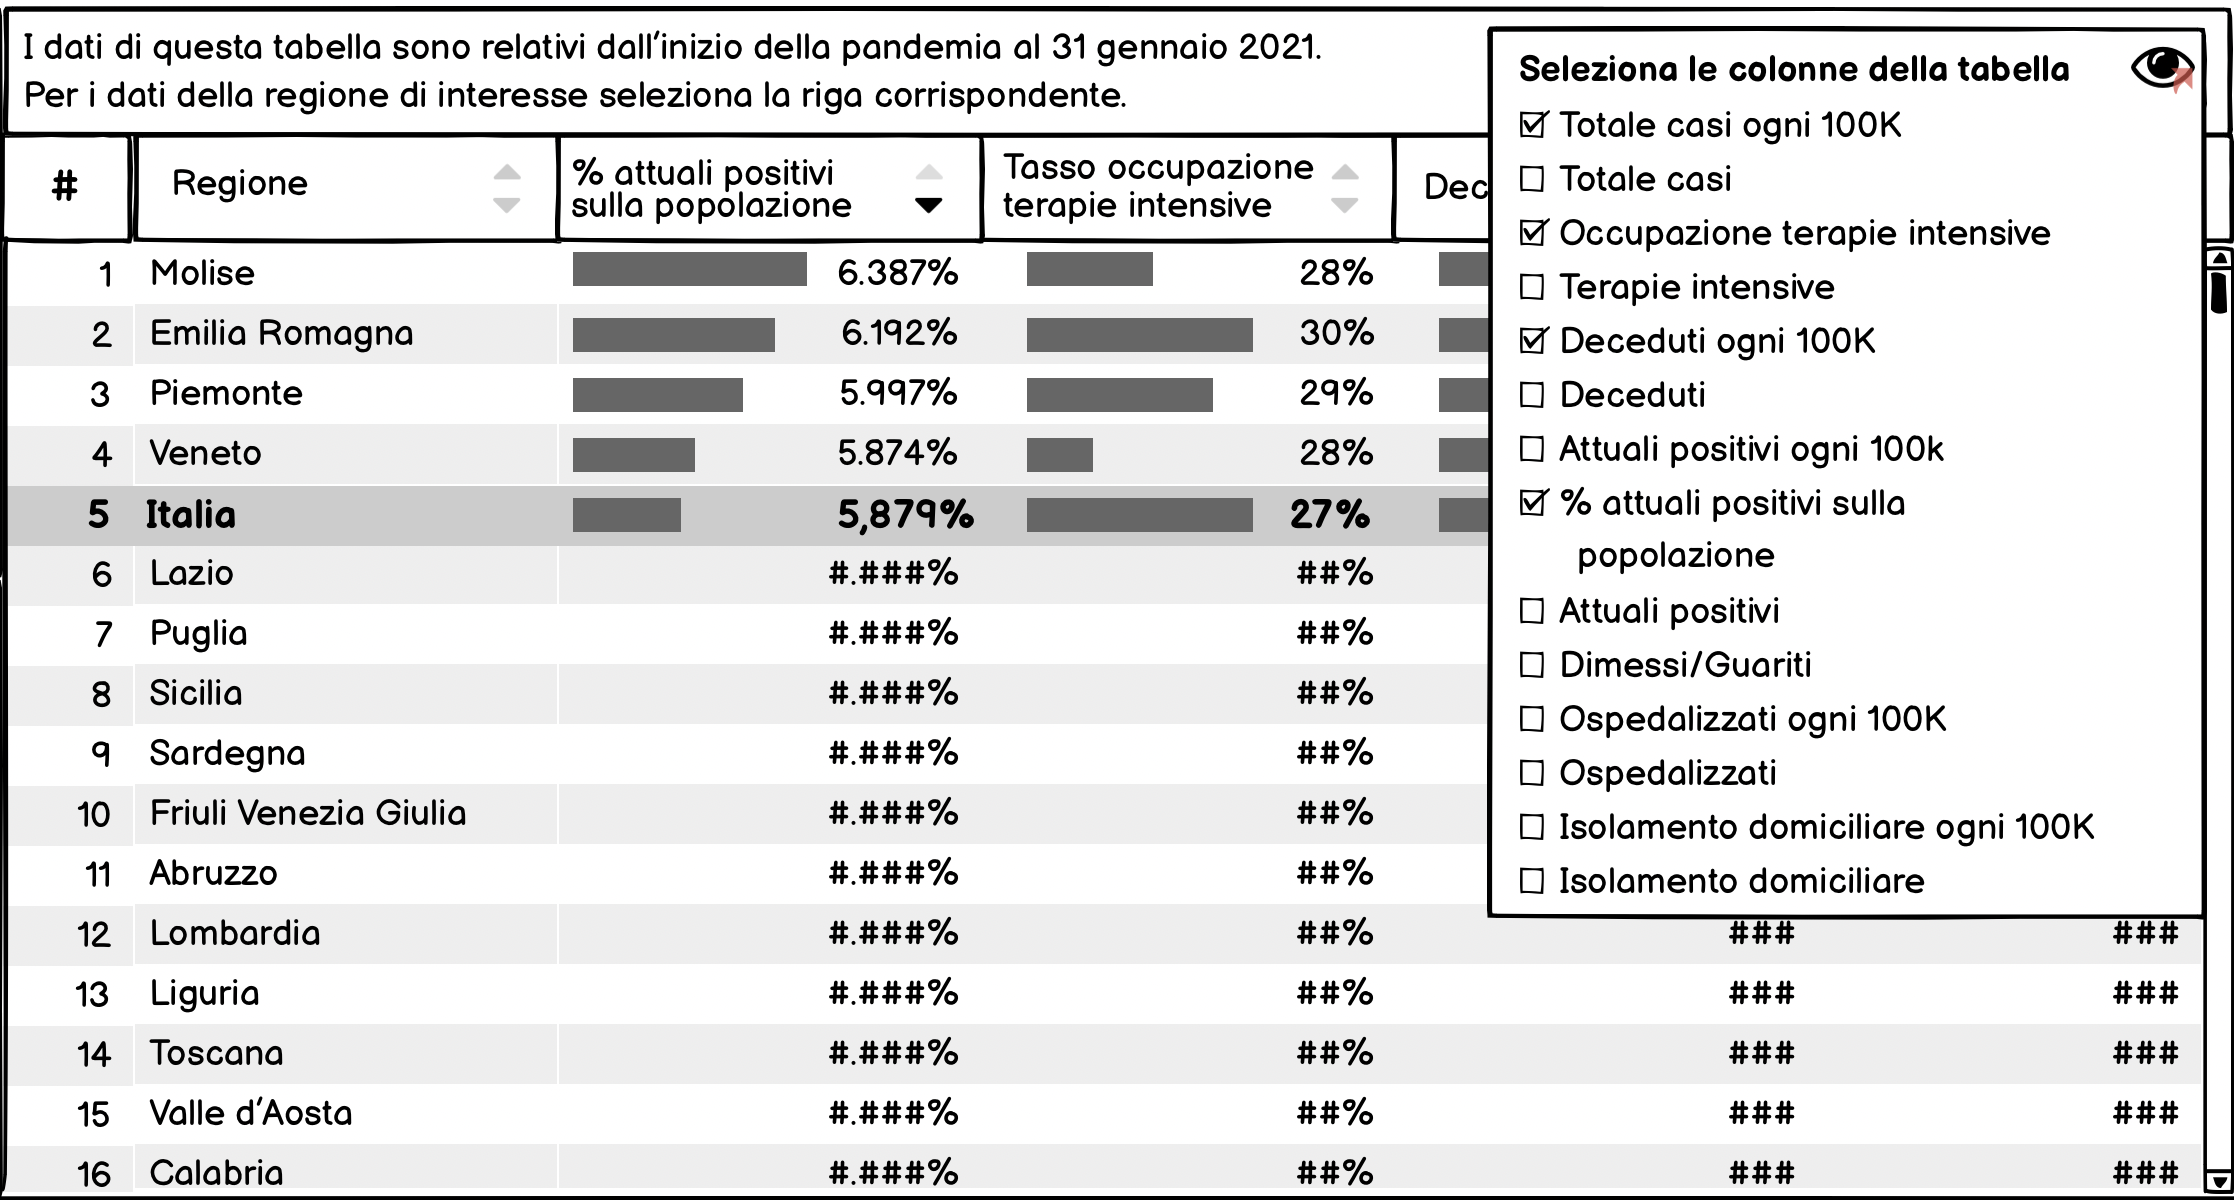
\includegraphics[width=0.7\columnwidth]{wireframes/lista-metriche-tabella}
    \caption{Lista delle metriche visionabili nella tabella.}
    \label{fig:lista-metriche-tabella}
\end{figure}

\begin{figure}[H]
    \centering
    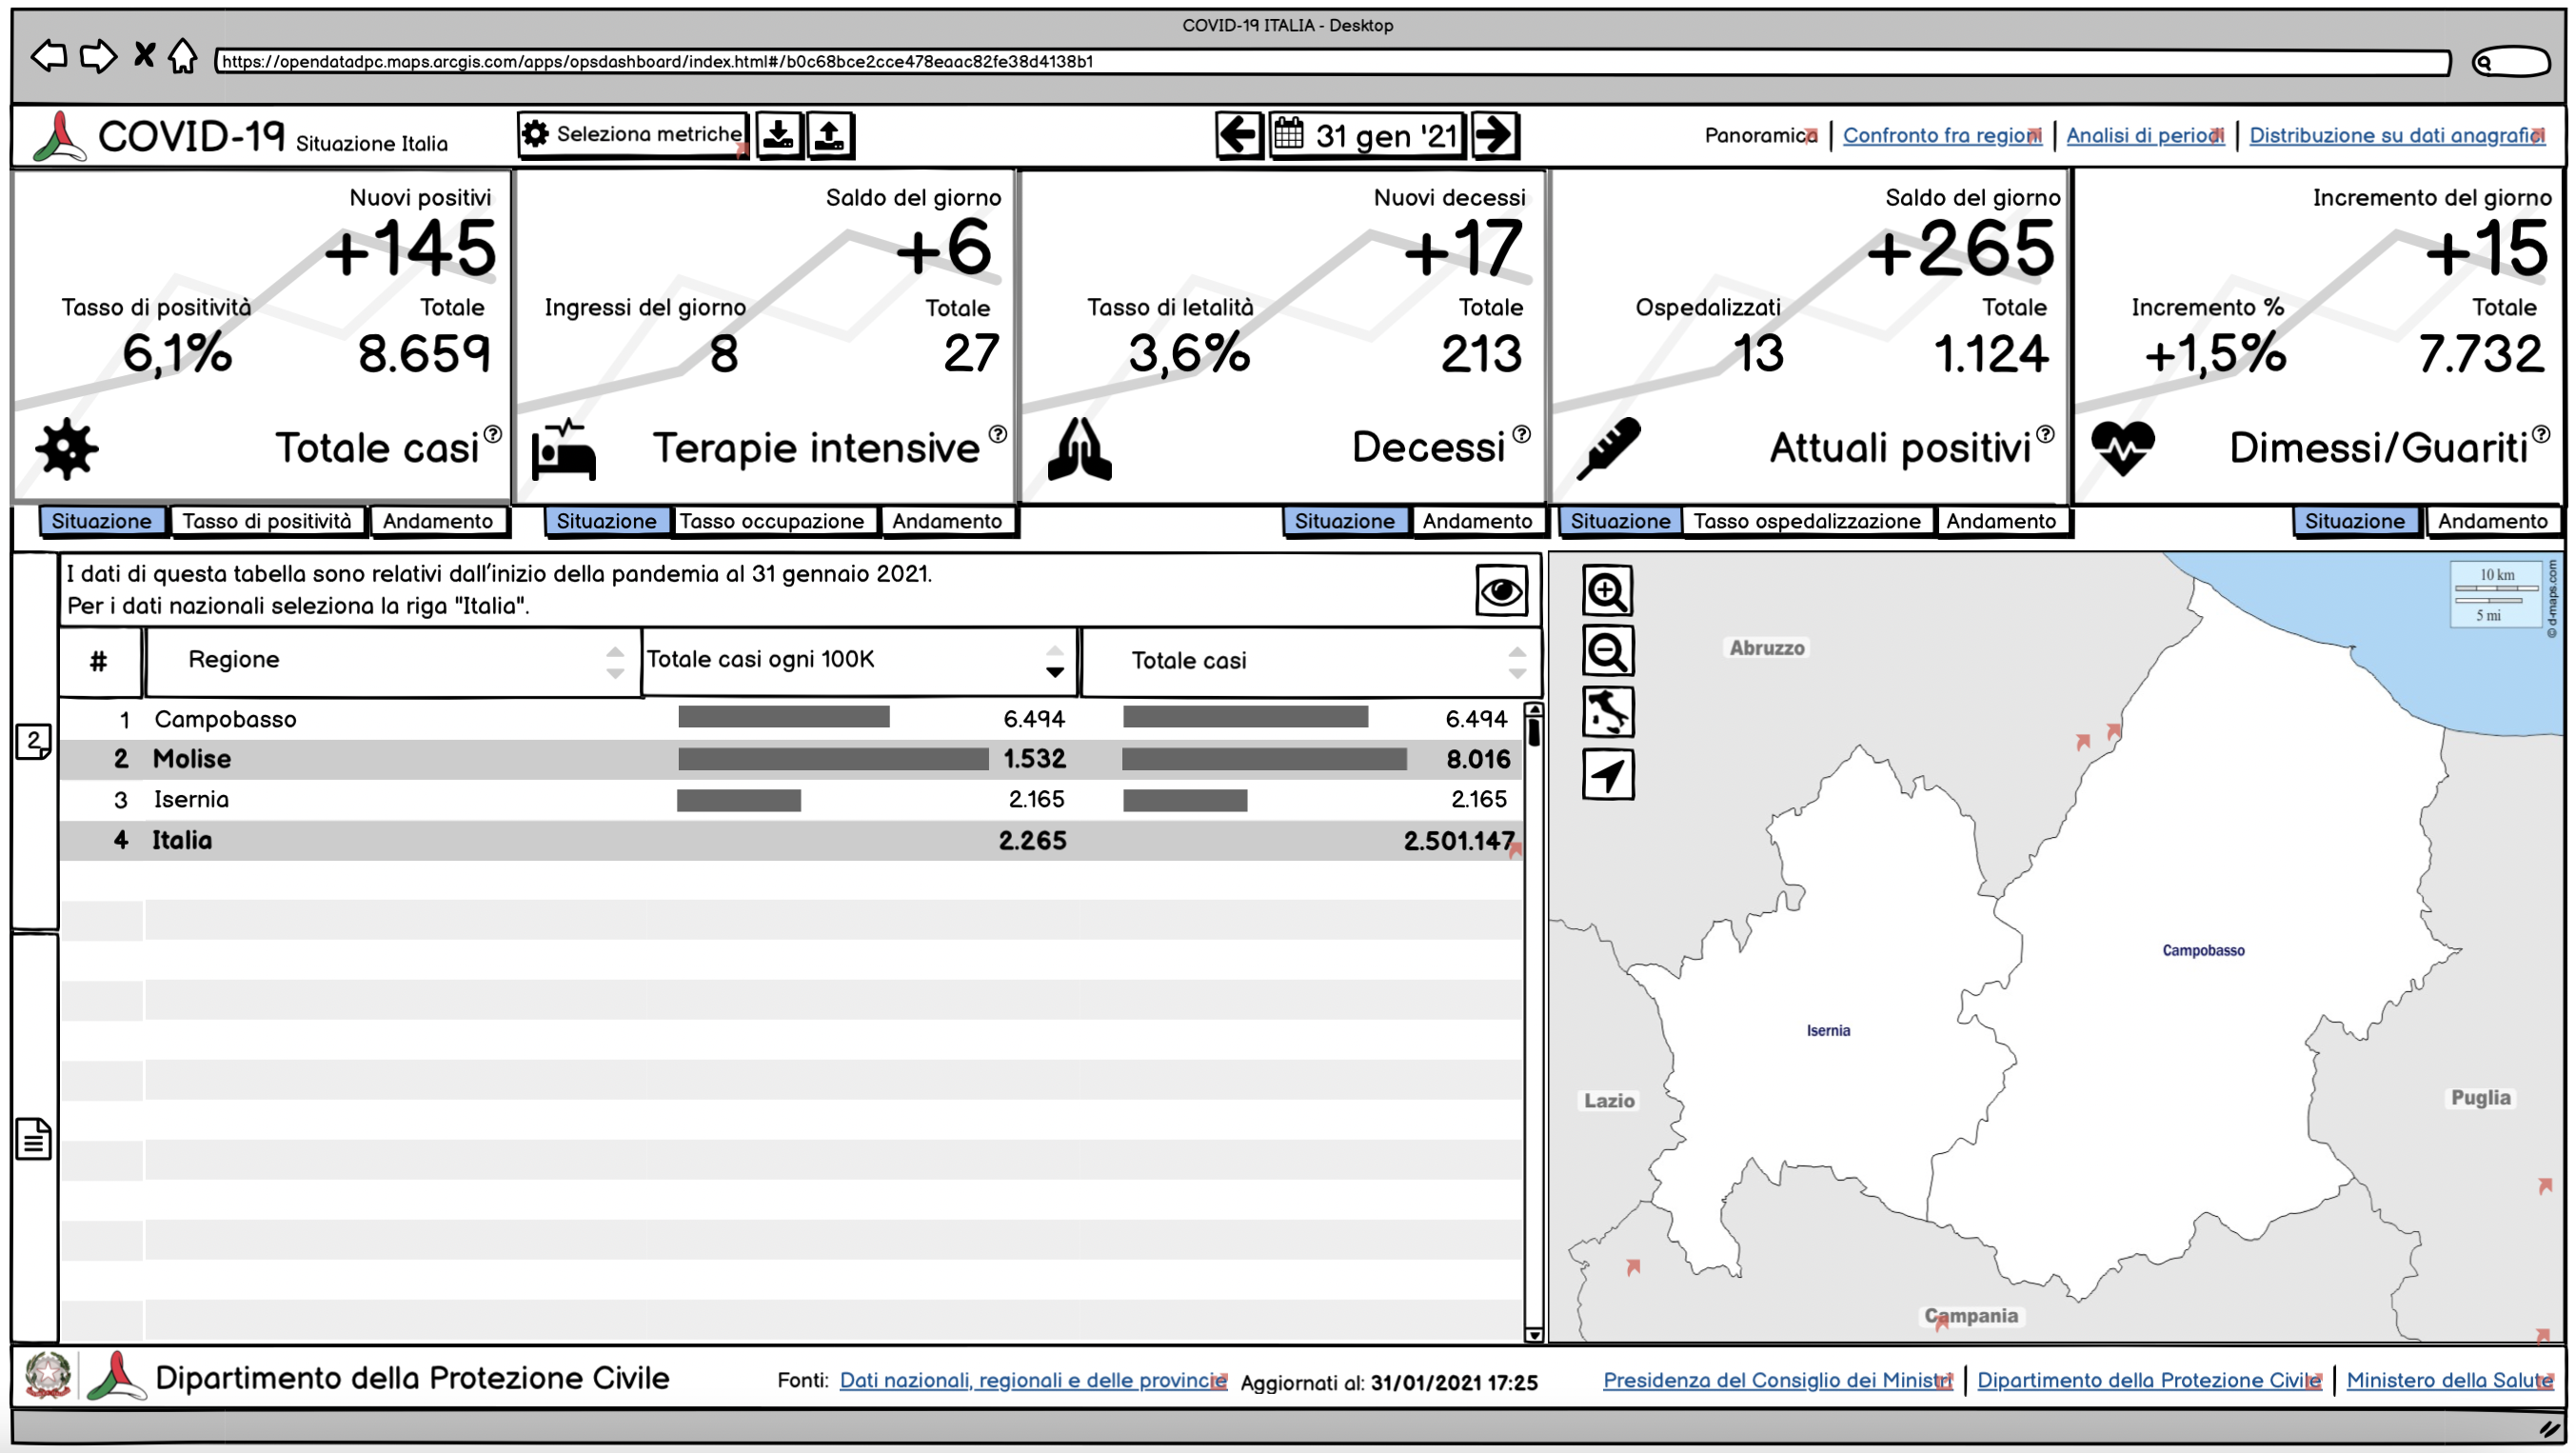
\includegraphics[width=0.7\columnwidth]{wireframes/panoramica-regione}
    \caption{Panoramica della regione Molise.}
    \label{fig:panoramica-regione}
\end{figure}
\clearpage
\paragraph{Mappa}\mbox{}\\
La mappa (Figura \ref{fig:mappa-panoramica}) è uno strumento utile per avere un colpo d'occhio sulla situazione dell'Italia o di una singola regione rispetto a una specifica metrica: quest'ultima è modificabile cliccando sulla ghiera in alto a destra, al cui click si apre una lista di metriche (Figura \ref{fig:lista-metriche-mappa}).
\begin{figure}[H]
    \begin{subfigure}[b]{0.5\textwidth}
        \centering
    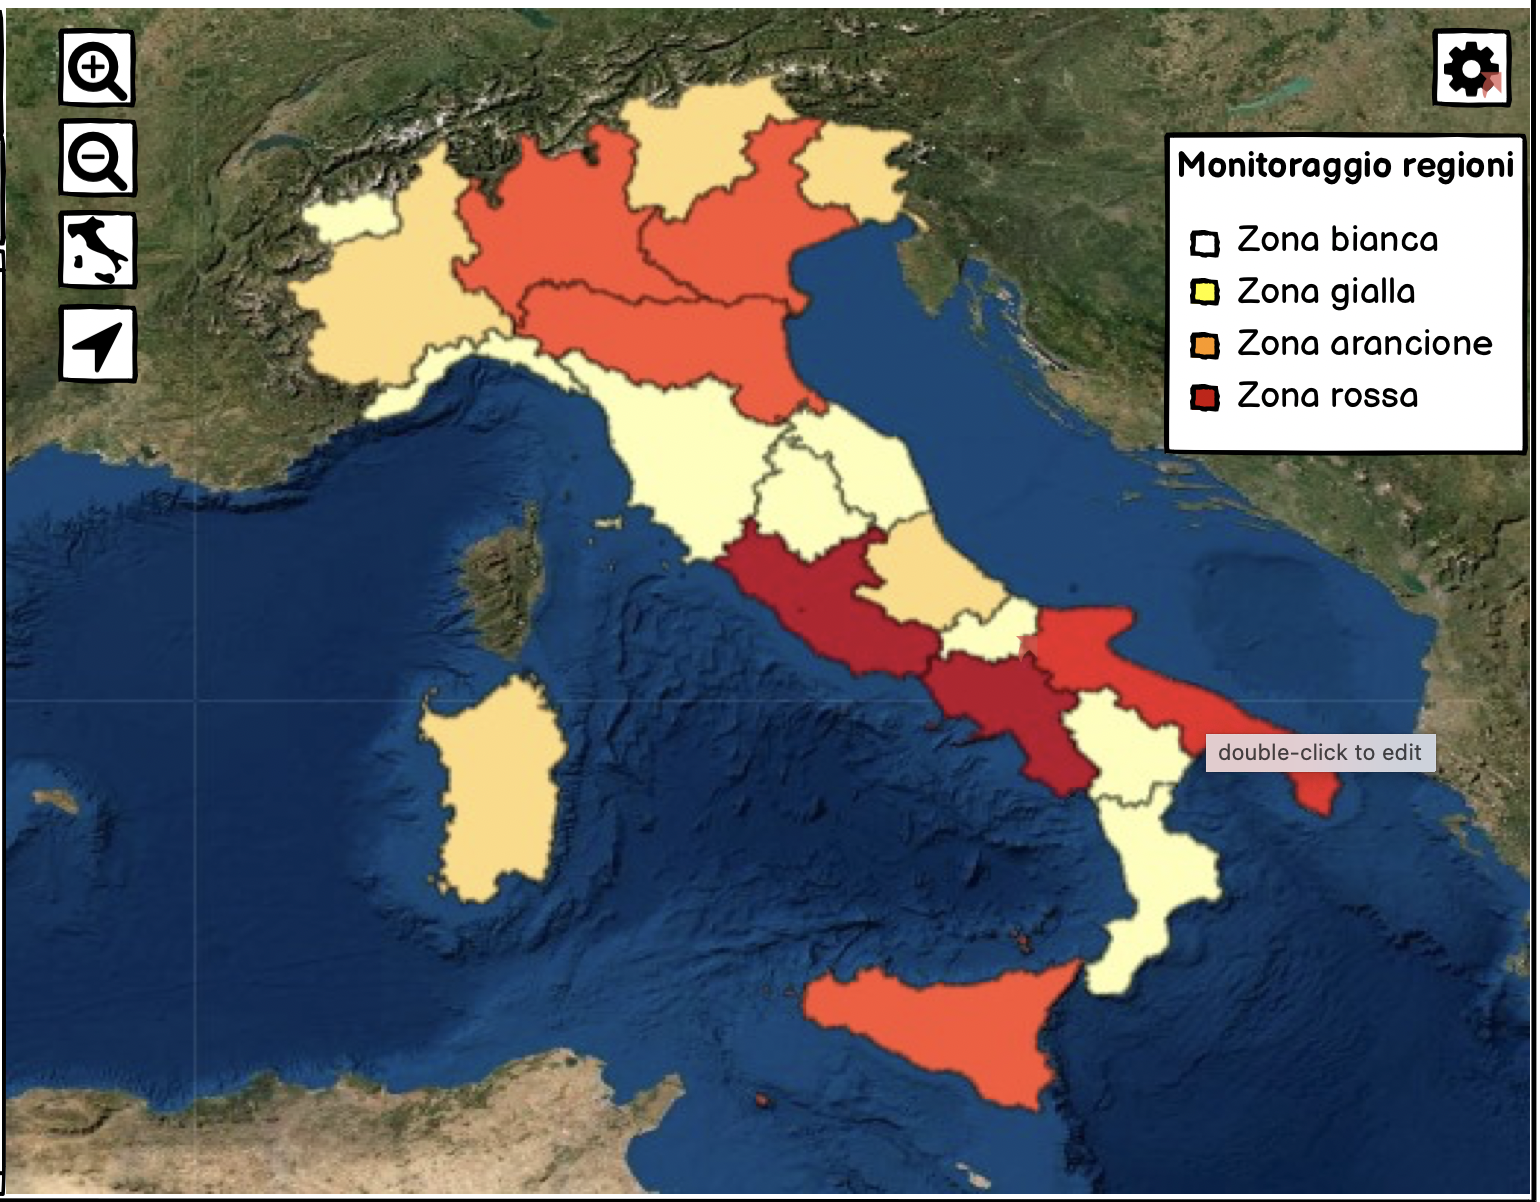
\includegraphics[width=0.7\columnwidth]{wireframes/mappa-panoramica}
    \caption{Heat map dell'Italia in ``Panoramica''.}
    \label{fig:mappa-panoramica}
    \end{subfigure}
    \hfill
    \begin{subfigure}[b]{0.5\textwidth}
        \centering
        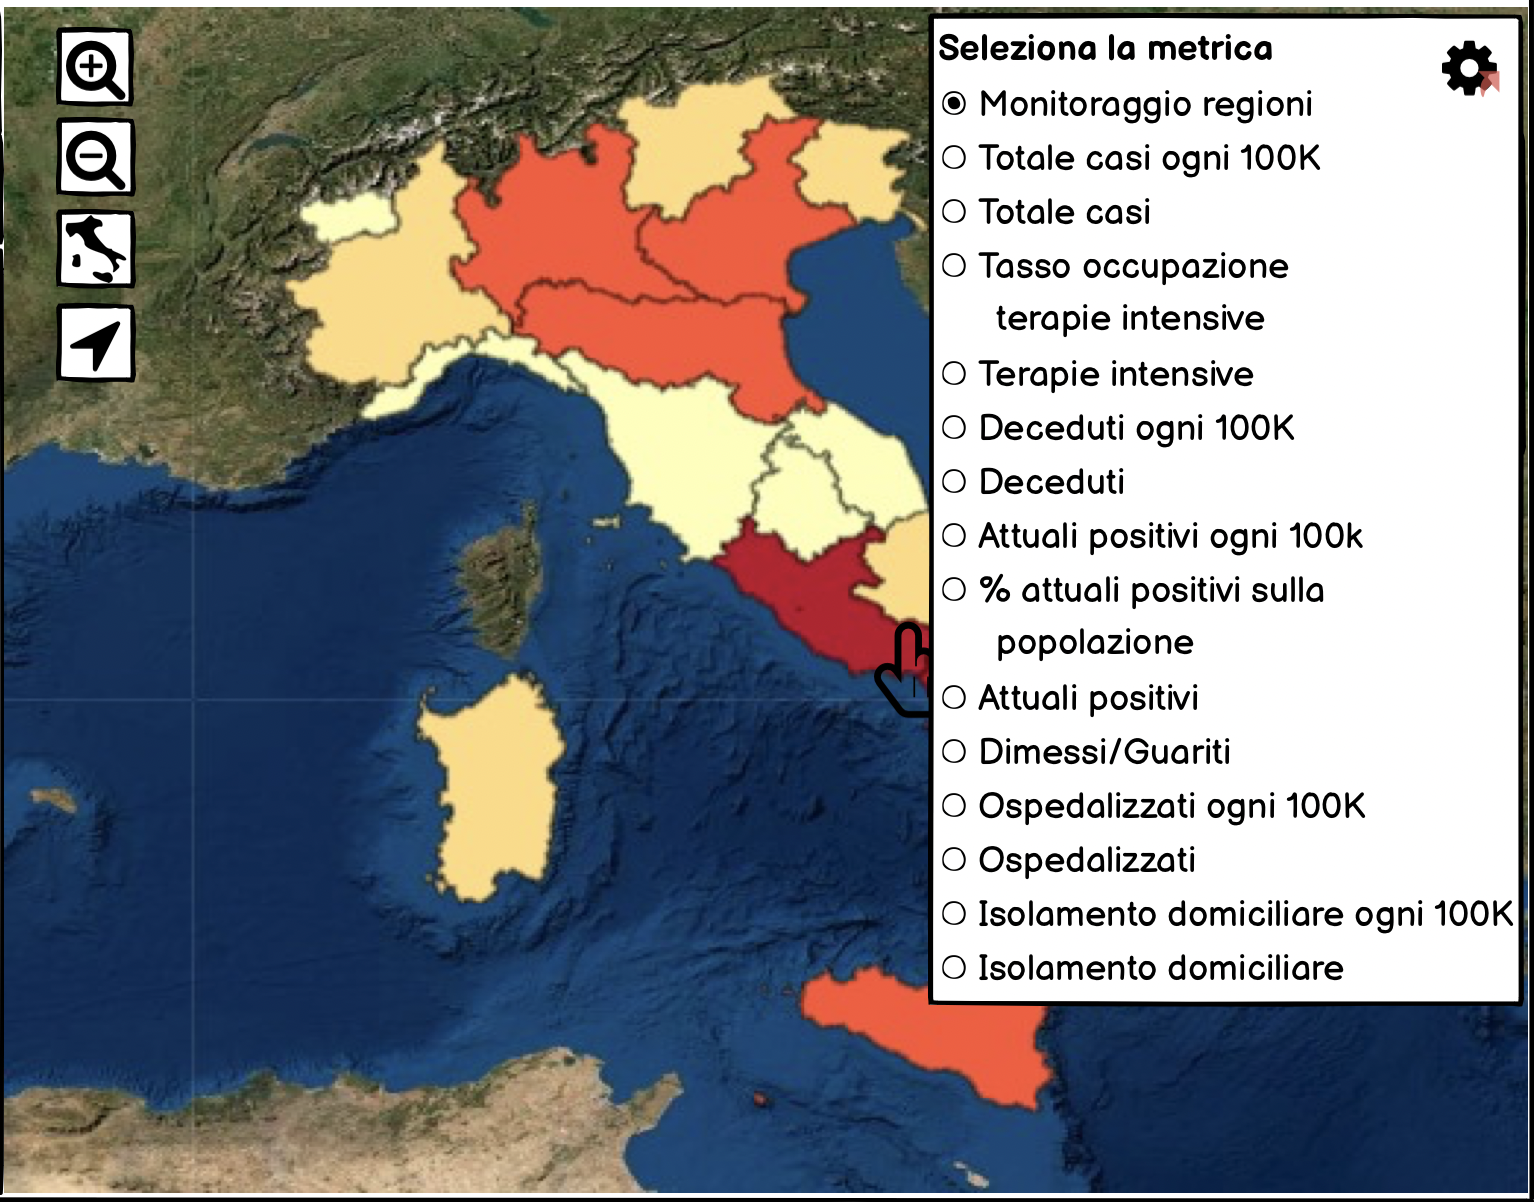
\includegraphics[width=0.7\columnwidth]{wireframes/lista-metriche-mappa}
        \caption{Lista delle metriche disponibili per la heat map.}
        \label{fig:lista-metriche-mappa}
    \end{subfigure}
\end{figure}
\noindent
Oltre alle interazioni possibili nella tabella, cliccando sull'area di regione nella mappa è possibile passare alla vista regionale della schermata ``Panoramica'' come in Figura \ref{fig:panoramica-regione}, mentre per tornare alla panoramica nazionale è possibile cliccare al di fuori dei confini regionali nella mappa.

\paragraph{Caricamento dei dati}\mbox{}\\
Abbiamo previsto una schermata di caricamento in attesa che i dati vengano scaricati e computati prima di essere mostrati; abbiamo usato degli spinner per indicare ciò.
\begin{figure}[H]
    \centering
    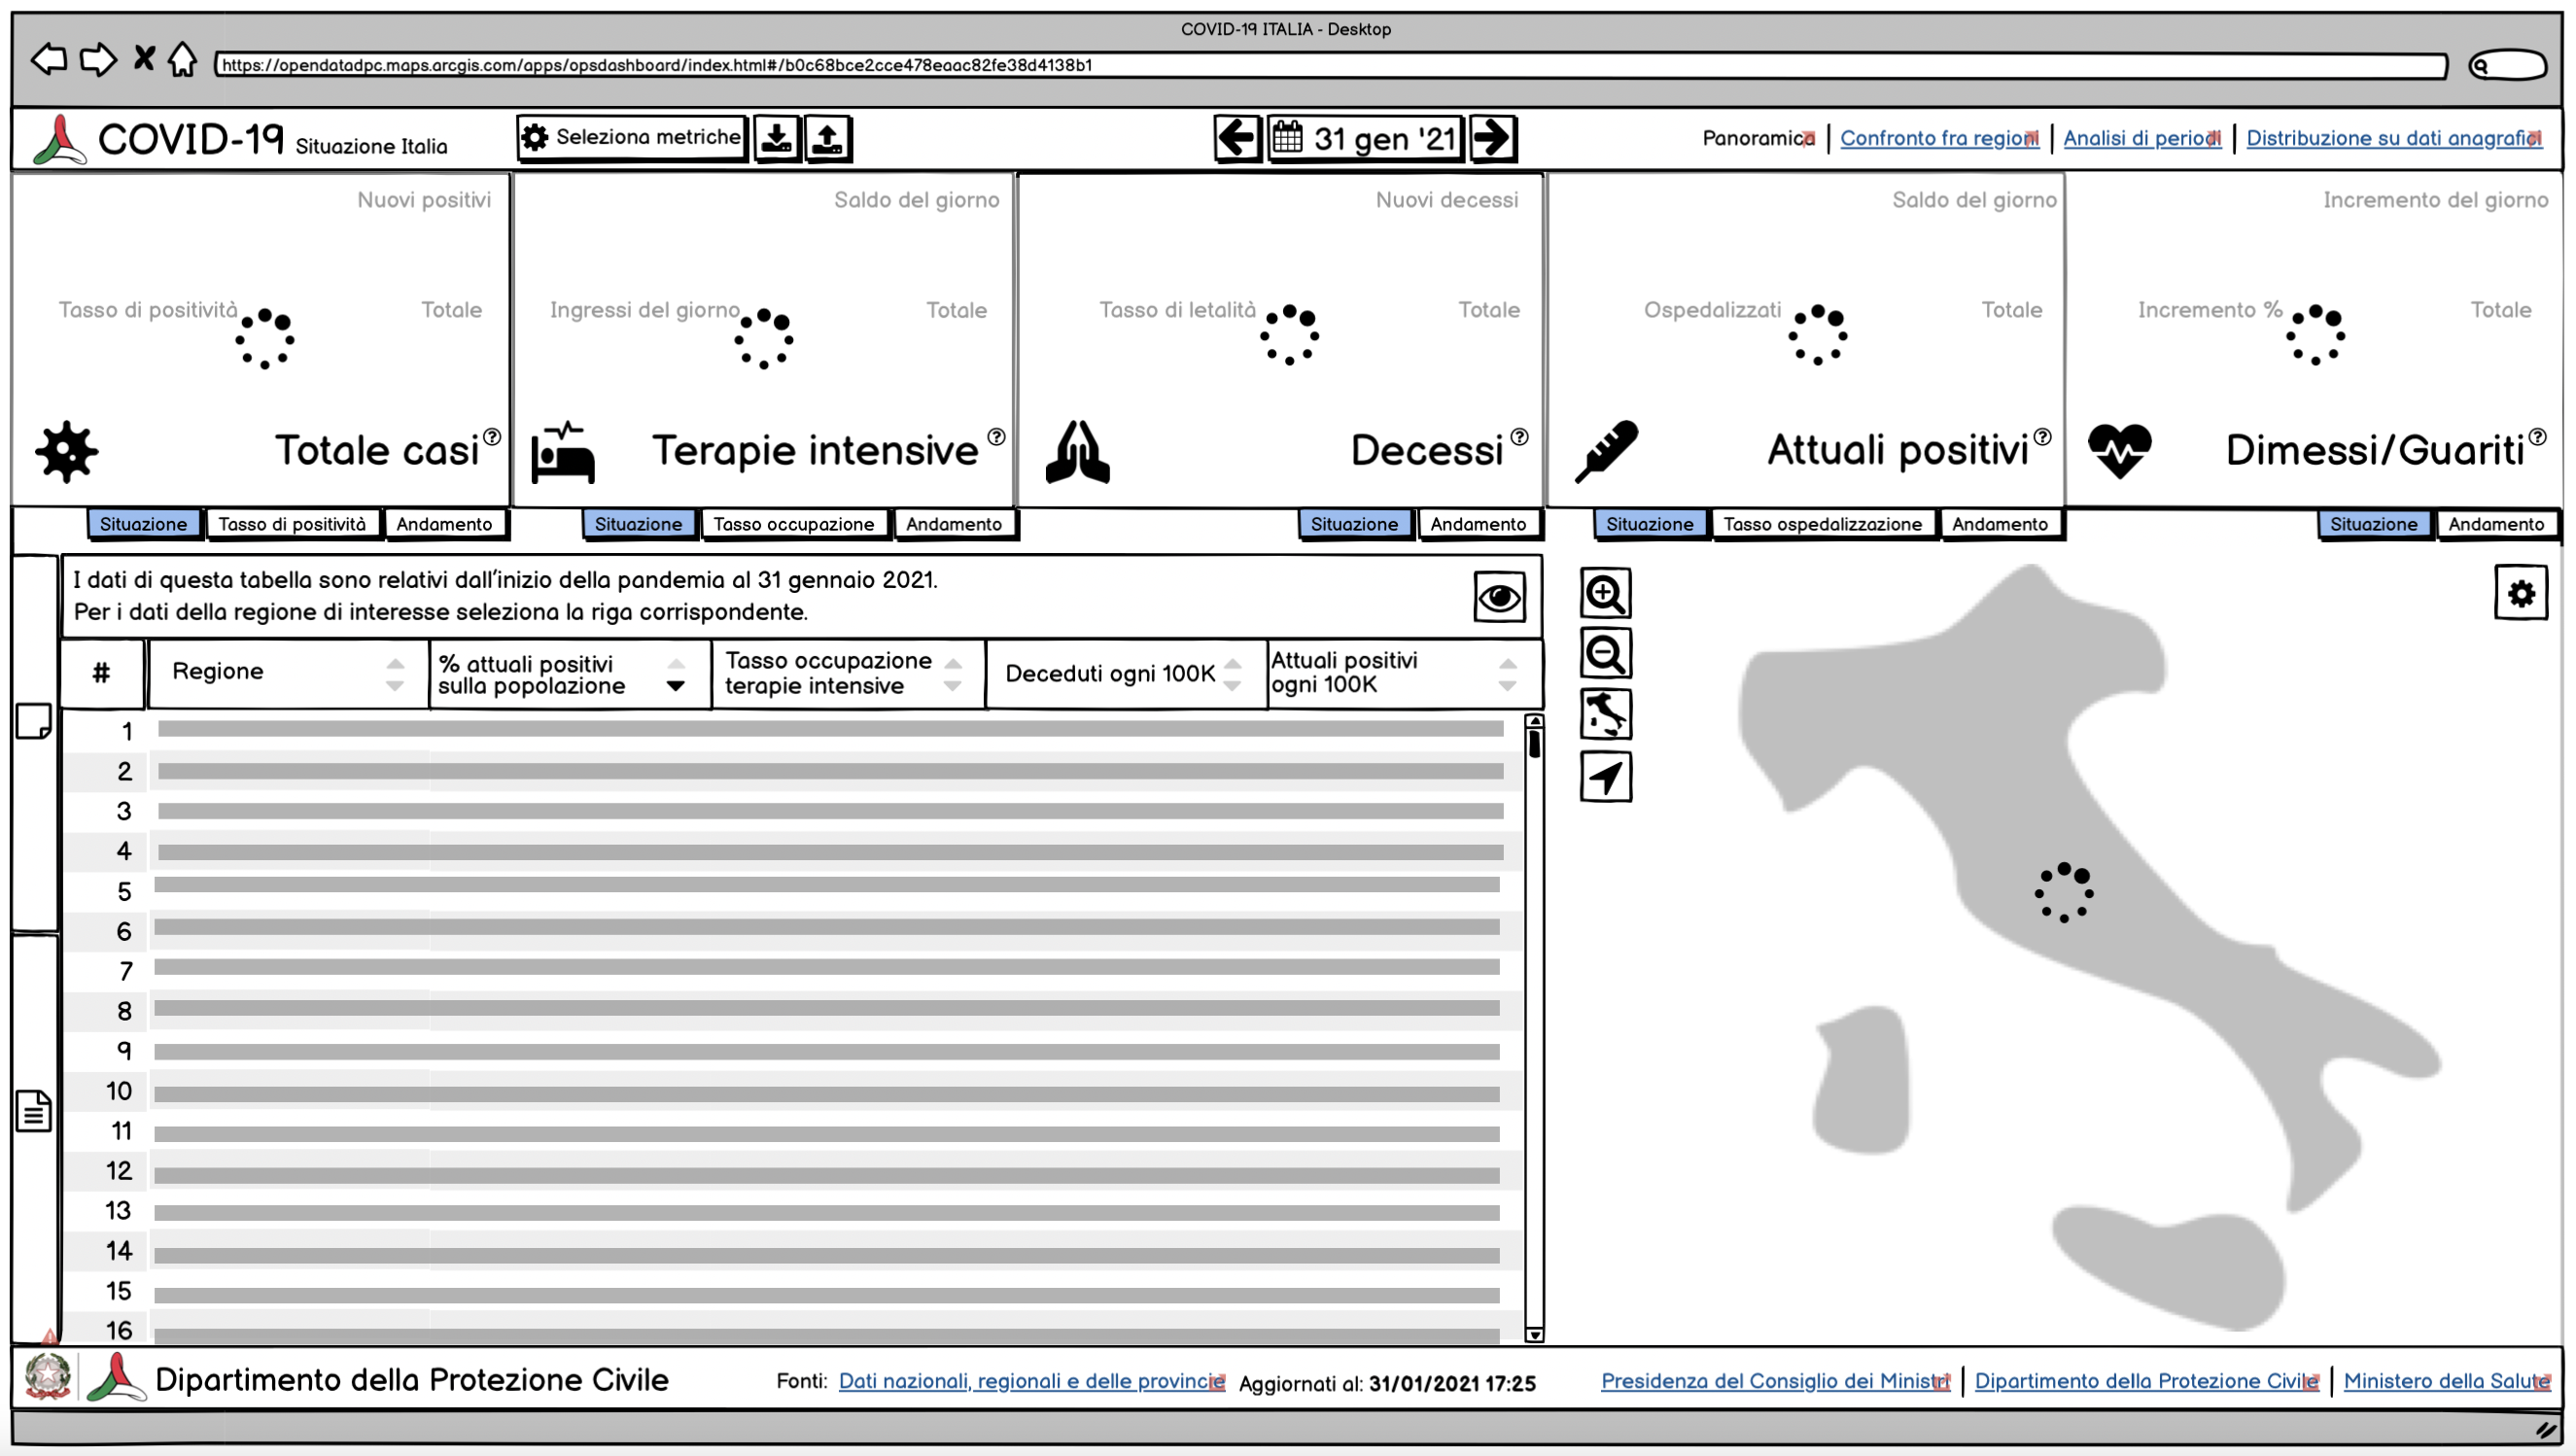
\includegraphics[width=.8\columnwidth]{wireframes/panoramica-caricamento}
    \caption{Schermata ``Panoramica'' durante il caricamento dei dati.}
    \label{fig:panoramica-caricamento}
\end{figure}

\subsubsection{Confronto fra regioni}\label{ss:confronto-fra-regioni}
\begin{figure}[H]
    \centering
    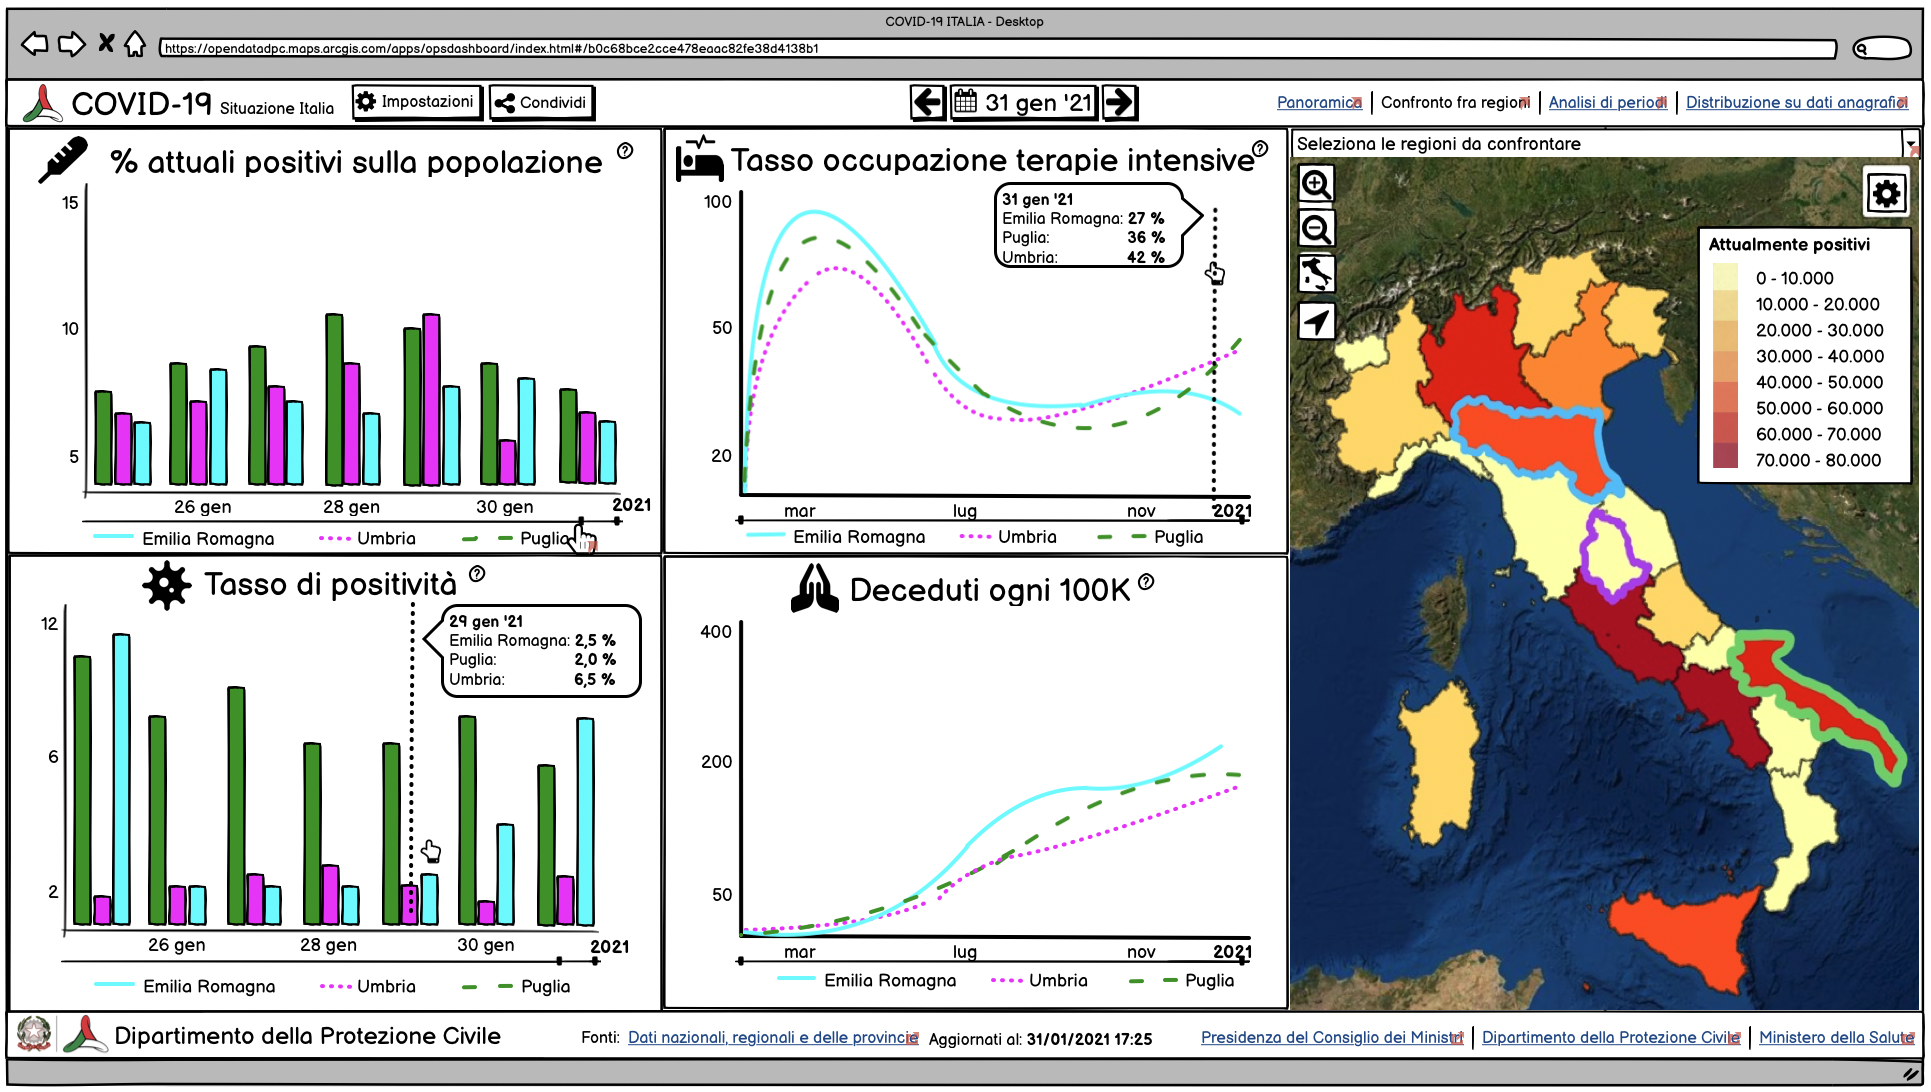
\includegraphics[width=1\columnwidth]{wireframes/confronto-regioni}
    \caption{Schermata ``Confronto fra regioni''.}
    \label{fig:confronto-regioni}
\end{figure}
La schermata ``Confronto fra regioni'' è raggiungibile cliccando sul link omonimo in alto a destra. In questa schermata è possibile selezionare una o più regioni per confrontare alcune metriche mediante dei grafici. La selezione avviene per mezzo una lista \textit{combo-box} posizionata al di sopra della mappa, come mostrato in Figura \ref{fig:seleziona-regione}, oppure cliccando direttamente sull'area della regione che si vuole aggiungere al confronto. Le regione selezionate sono indicate tramite una spunta (\checkmark) e i loro confini sono colorati con gli stessi colori assunti poi nei grafici.

\begin{figure}[H]
    \centering
    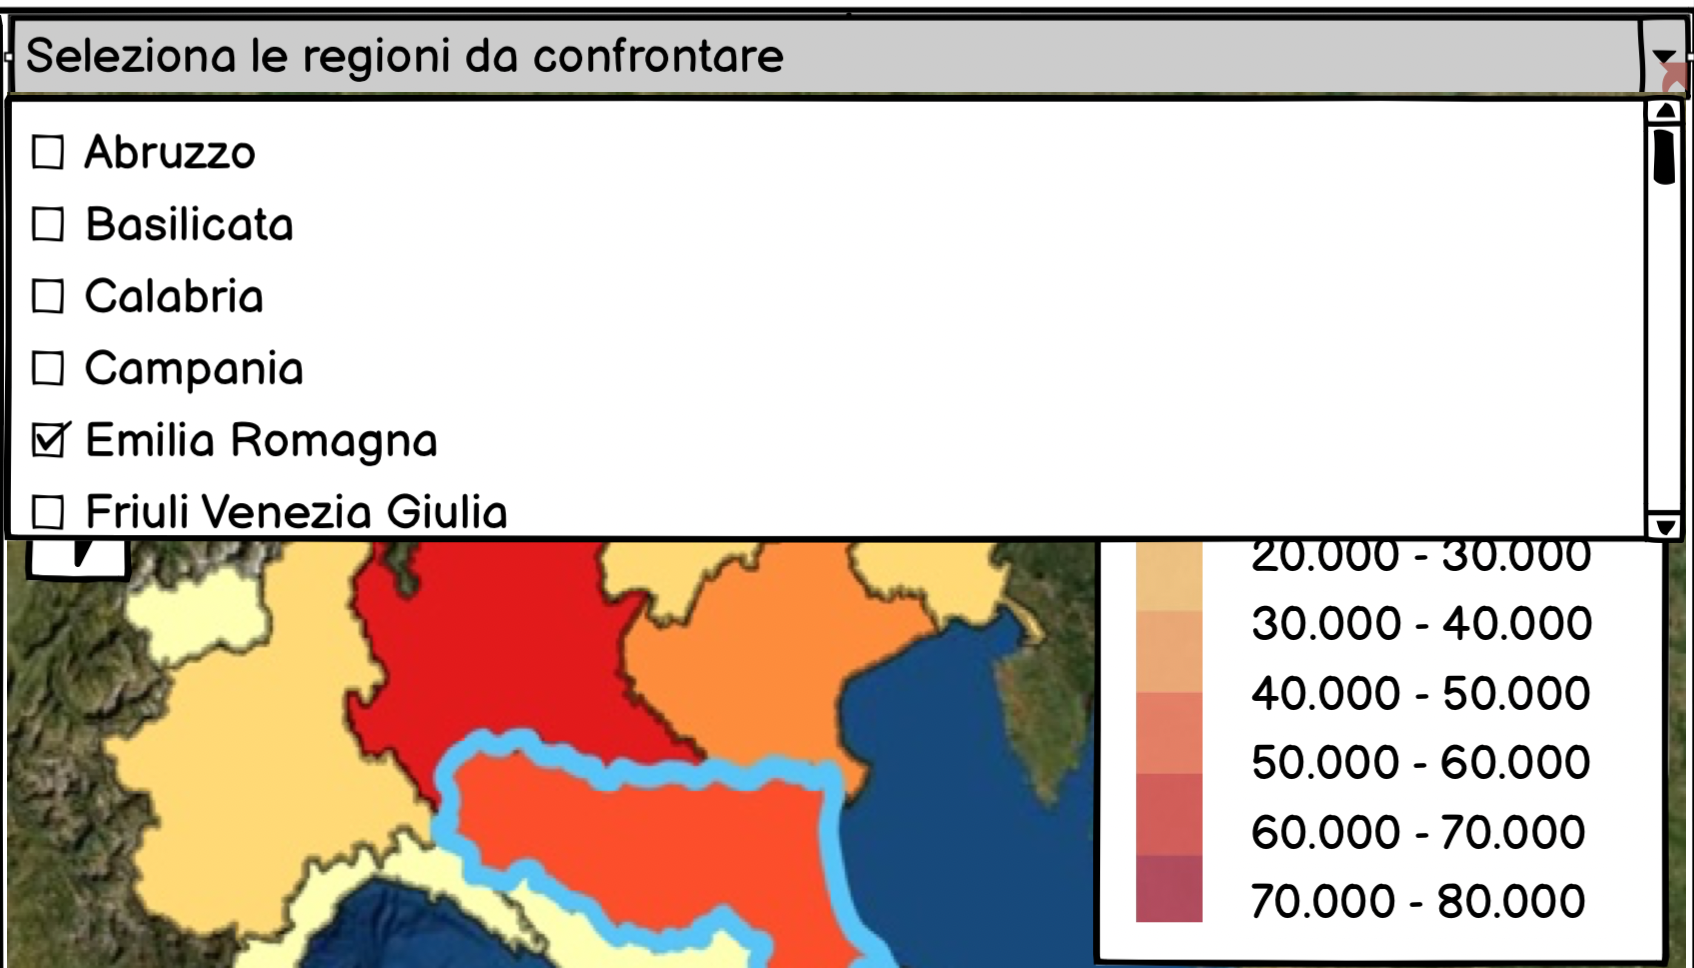
\includegraphics[width=0.5\columnwidth]{wireframes/seleziona-regione}
    \caption{Combo-box per la selezione delle regioni.}
    \label{fig:seleziona-regione}
\end{figure}
\noindent
I grafici presenti sulla parte sinistra della schermata, di cui Figura \ref{fig:esempio-grafico-confronto-regioni} ne è un esempio, sono formati da una curva per ogni regione selezionata: le curve sono distinte tanto per colore quanto per tipo di tratteggio, cosicché la distinzione è chiara anche ai soggetti aventi difficoltà nel riconoscere i colori.

\begin{figure}[H]
    \begin{subfigure}[b]{0.5\textwidth}
        \centering
        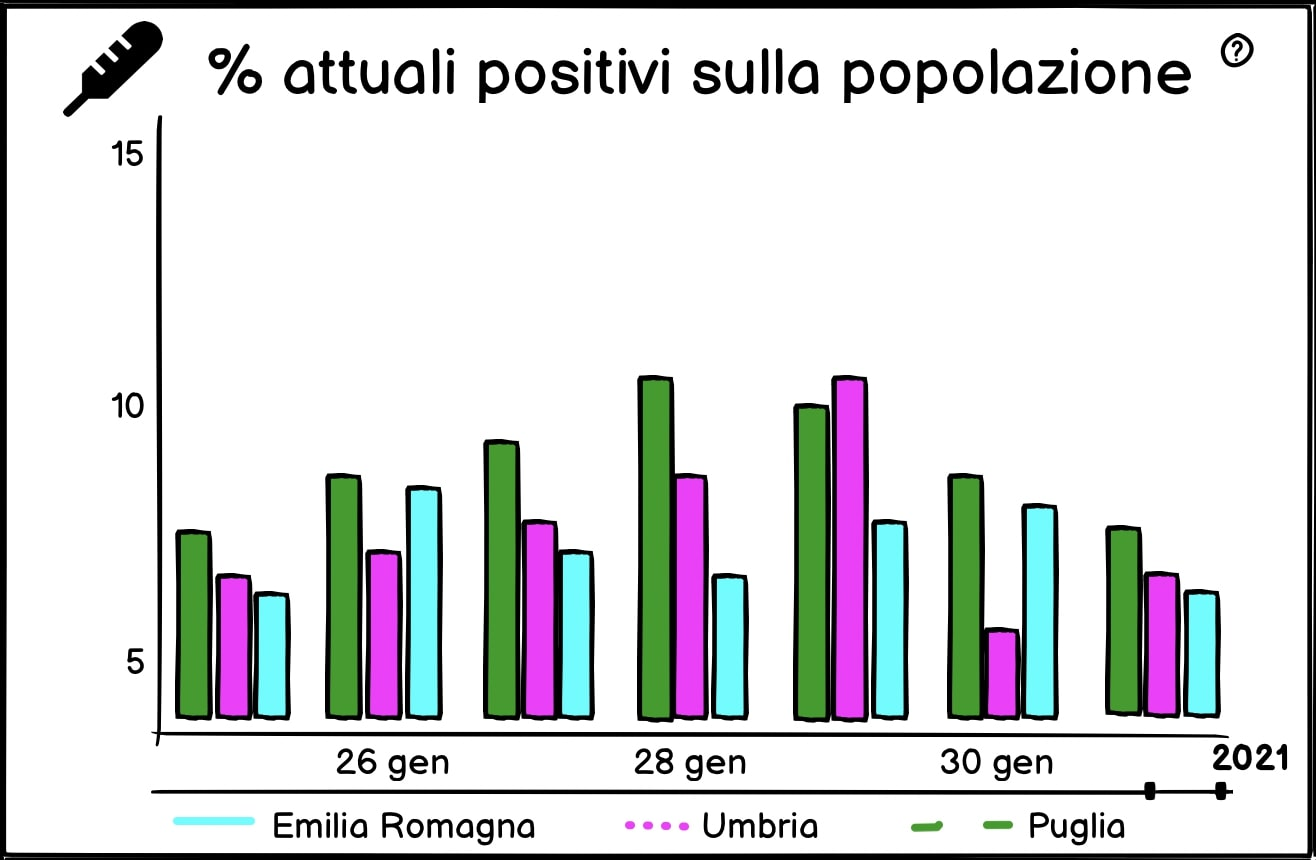
\includegraphics[width=1\textwidth]{wireframes/esempio-grafico-confronto-regioni-poco-tempo}
        \caption{Grafico per il quale è stato selezionato un range temporale di breve durata.}
        \label{fig:esempio-grafico-confronto-regioni-poco-tempo}
    \end{subfigure}
\hfill
    \begin{subfigure}[b]{0.45\textwidth}
        \centering
        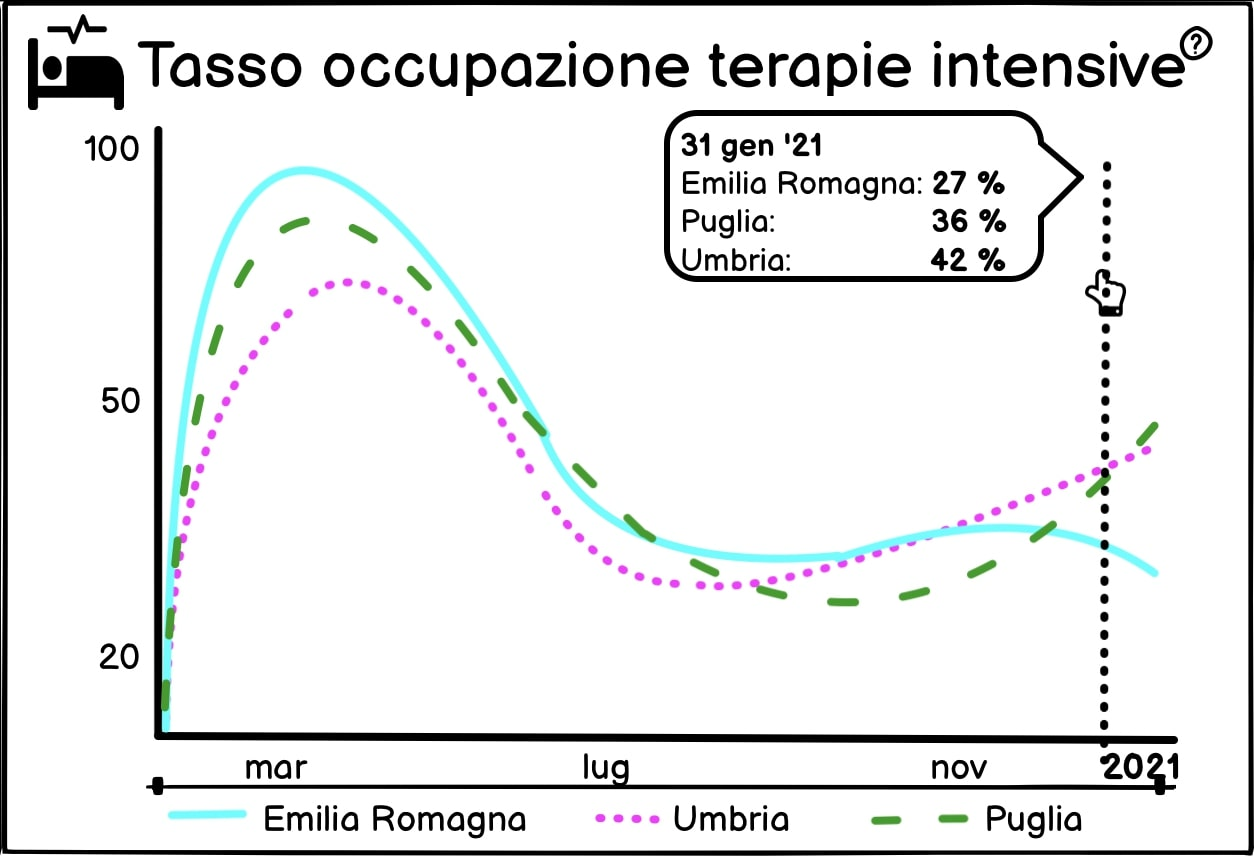
\includegraphics[width=1\textwidth]{wireframes/esempio-grafico-confronto-regioni-molto-tempo}
        \caption{Grafico per il quale è selezionato un range temporale di lunga durata.}\label{fig:esempio-grafico-confronto-regioni-molto-tempo}
    \end{subfigure}
    \caption{Differenze tra un grafico in cui è selezionato un range di tempo di breve durata e uno di lunga.}
    \label{fig:esempio-grafico-confronto-regioni}
\end{figure}
\clearpage
\subsubsection{Analisi di periodi}\label{ss:analisi-di-periodi}
\begin{figure}[H]
    \centering
    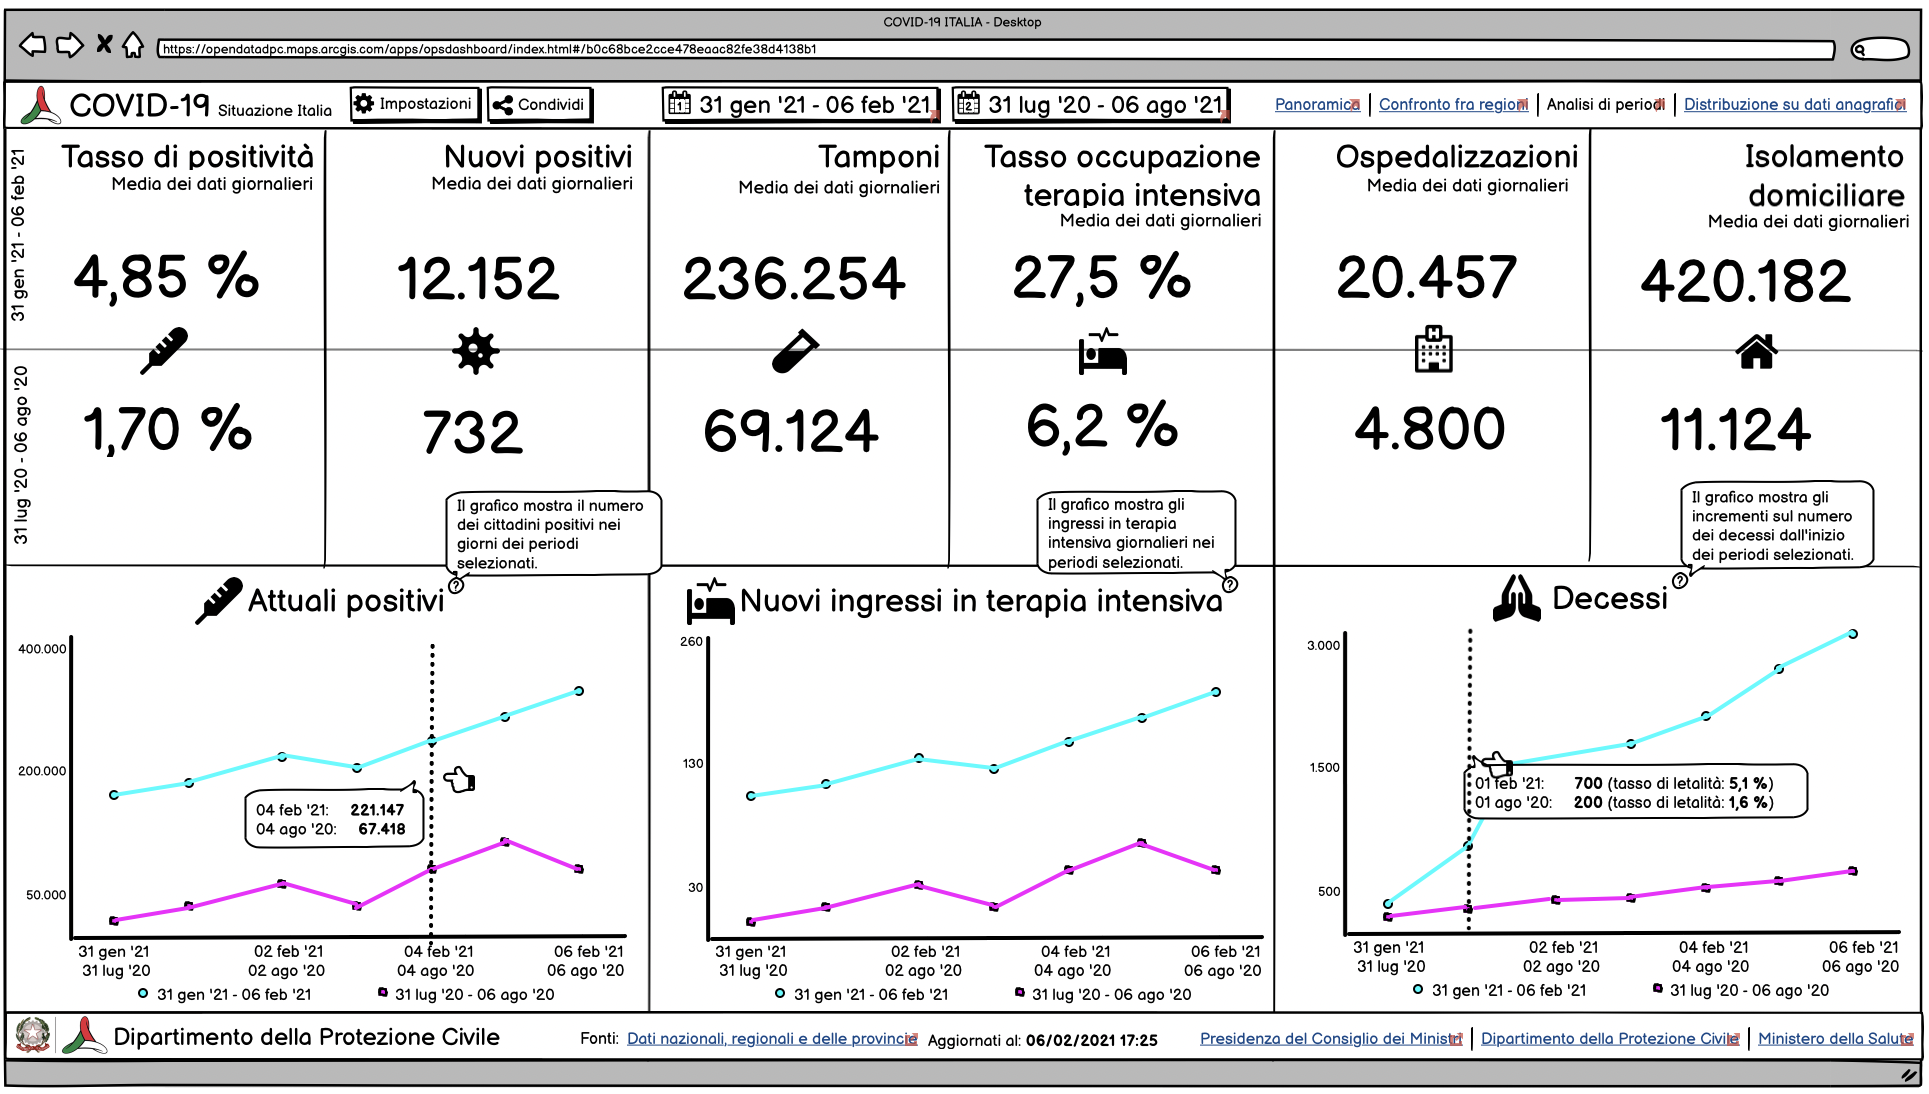
\includegraphics[width=1\columnwidth]{wireframes/new-analisi-periodi}
    \caption{Schermata ``Analisi di periodi''.}
    \label{fig:analisi-periodi}
\end{figure}
La schermata ``Analisi di periodi'' è raggiungibile dal link omonimo in alto a destra. In questa schermata è possibile analizzare l'andamento della pandemia per uno o due periodi.\\
La schermata può, per semplicità, essere divisa in due fasce: nella fascia superiore vi è una componente assimilabile a una tabella, le cui righe sono relative ai periodi temporali specificati, e le cui colonne sono relative alle metriche d'interesse; i valori numerici che compaiono sono aggregati con riferimento alle finestre temporali indicate.\\
Nella parte inferiore della schermata trovano spazio tre grafici, i quali, sull'asse delle $x$, riportano i giorni dei periodi temporali che si stanno analizzando così da permettere un più semplice confronto.
\clearpage
\begin{bclogo}{Iterazioni in Analisi di periodi}
Prima di arrivare al design definitivo della schermata ``Analisi di periodi'' abbiamo considerato diverse possibilità.\\
Inizialmente pensavamo di mantenere un'organizzazione simile a quella già usata con dei box numerici (Figura \ref{fig:box-numerici-analisi-di-periodi-versione-1}). Ci siamo resi conto che così facendo avremmo ripetuto le date in ogni box e quindi questa prima soluzione ci è sembrata un po' troppo ridondante. Abbiamo quindi pensato di riorganizzare la schermata costruendo una specie di tabella (Figura \ref{fig:analisi-di-periodi-seconda-versione}) ma, in questo caso ci siamo immediatamente resi conto che lo spazio verticale veniva usato in maniera poco intelligente.
\begin{figure}[H]
    \centering
    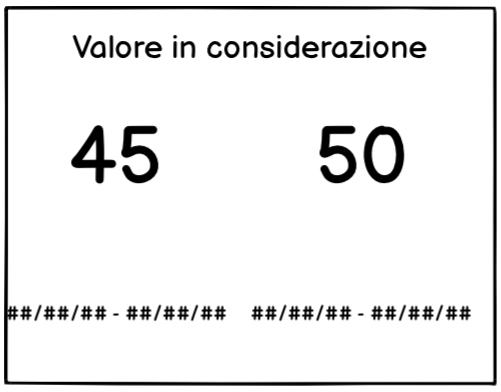
\includegraphics[width=0.3\columnwidth]{wireframes/box-numerici-analisi-di-periodi-versione-1}
    \caption{Prima versione del box numerico per confrontare i valori di una metrica in due periodi.}\label{fig:box-numerici-analisi-di-periodi-versione-1}
\end{figure}
\begin{figure}[H]
    \centering
    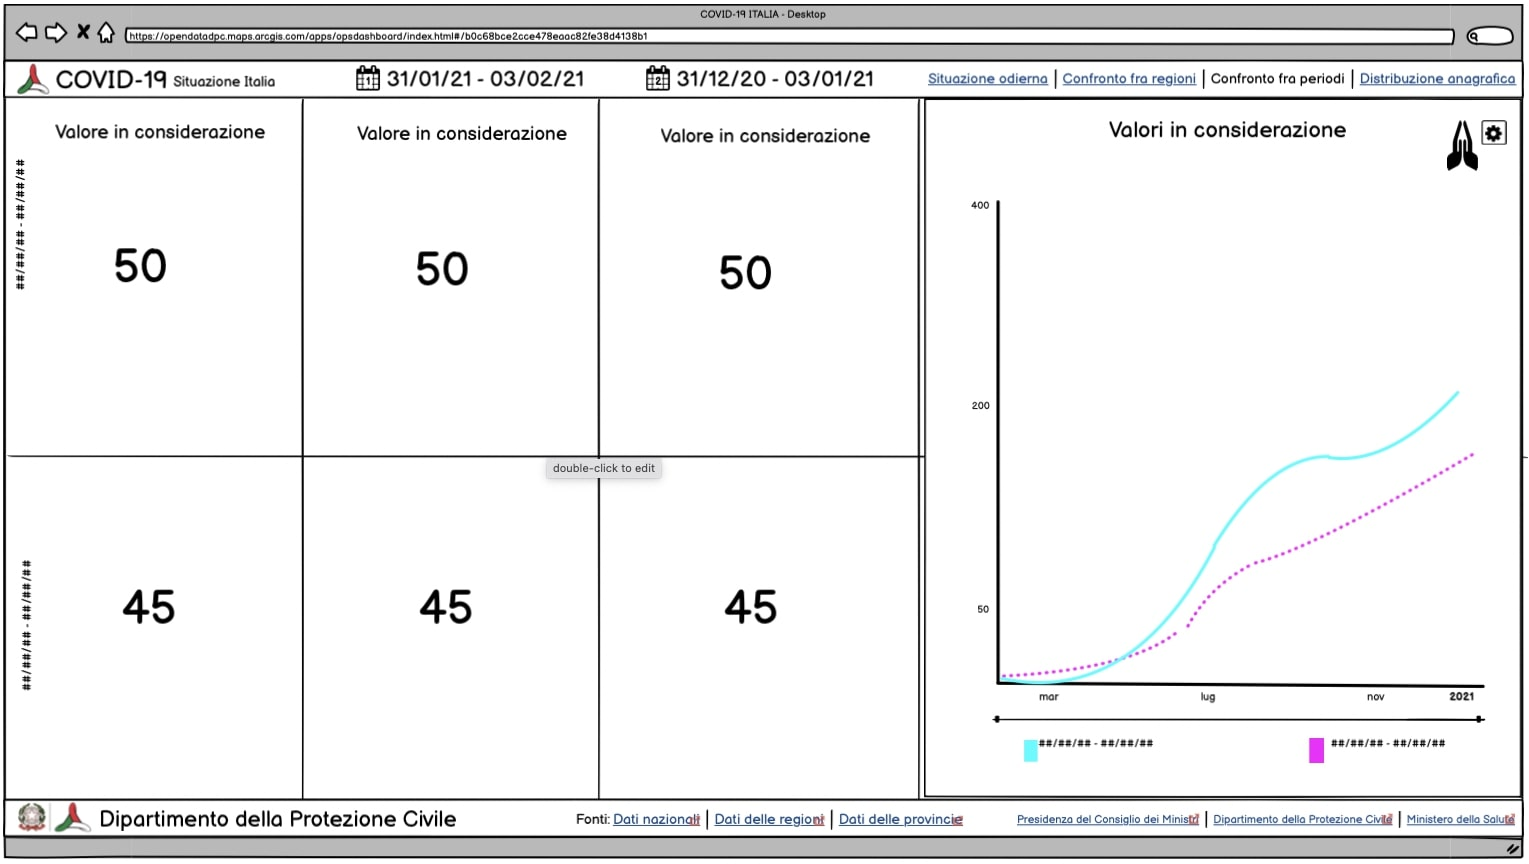
\includegraphics[width=0.7\columnwidth]{wireframes/analisi-di-periodi-seconda-versione}
    \caption{Versione scartata della schermata ``Analisi di periodi''.}
    \label{fig:analisi-di-periodi-seconda-versione}
\end{figure}
\noindent
Mantenendo per buona l'idea di ``tabella'' siamo giunti al design finale occupando la fascia in alto della schermata con una tabella e la fascia in basso con dei grafici.\\
\noindent
Dopo aver intervistato alcuni giornalisti abbiamo modificato il metodo con il quale visualizziamo i grafici quando i giorni selezionati sono pochi: nelle precedente versione (Figura \ref{fig:old-analisi-periodo}) mostravamo solamente i punti relativi ai giorni, questo ha destato confusione negli intervistati, abbiamo quindi decisi di aggiungere delle linee che collegano i vari punti; pur sapendo essere matematicamente scorretto non essendo dati continui, abbiamo optato per questa soluzione in quanto si è rivelata essere più chiara per gli utenti.
\begin{figure}[H]
    \centering
    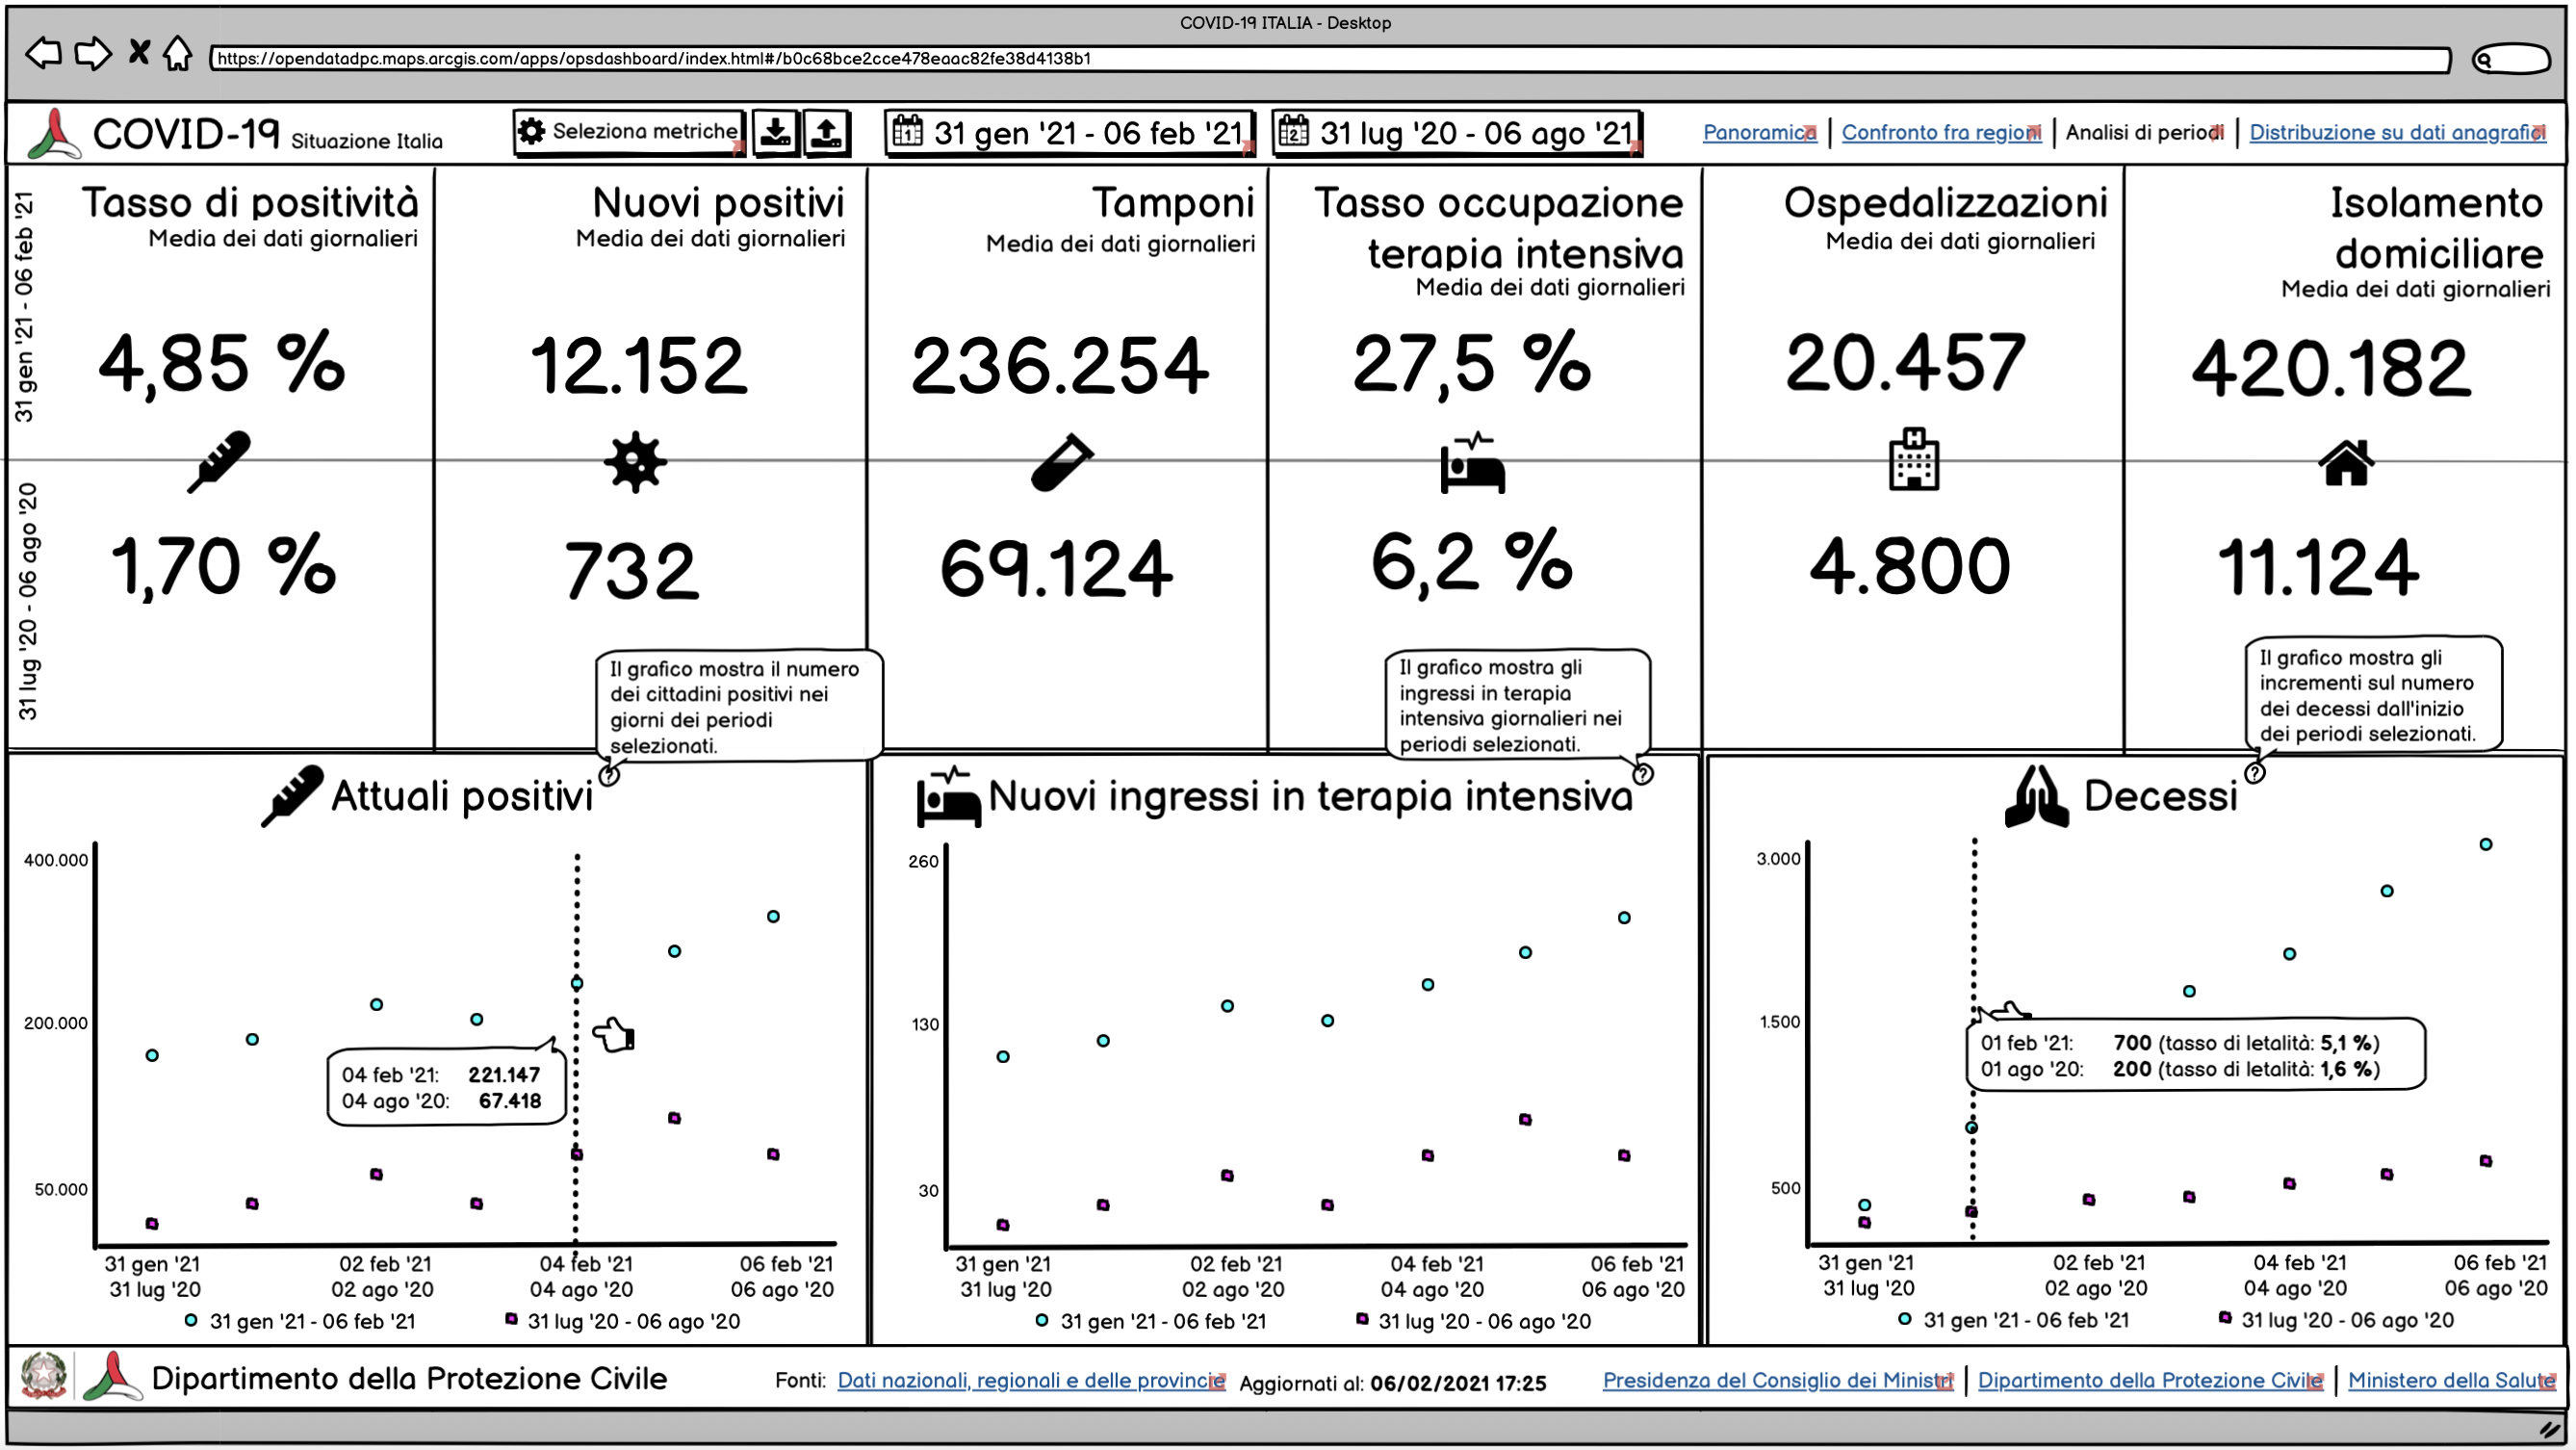
\includegraphics[width=0.7\columnwidth]{wireframes/analisi-periodi}
    \caption{Versione scartata con grafici a punti della schermata ``Analisi di periodi''.}
    \label{fig:old-analisi-periodo}
\end{figure}
\end{bclogo}
\clearpage
\subsubsection{Distribuzione su dati anagrafici}\label{ss:distribuzione-su-dati-anagrafici}
\begin{figure}[H]
    \centering
    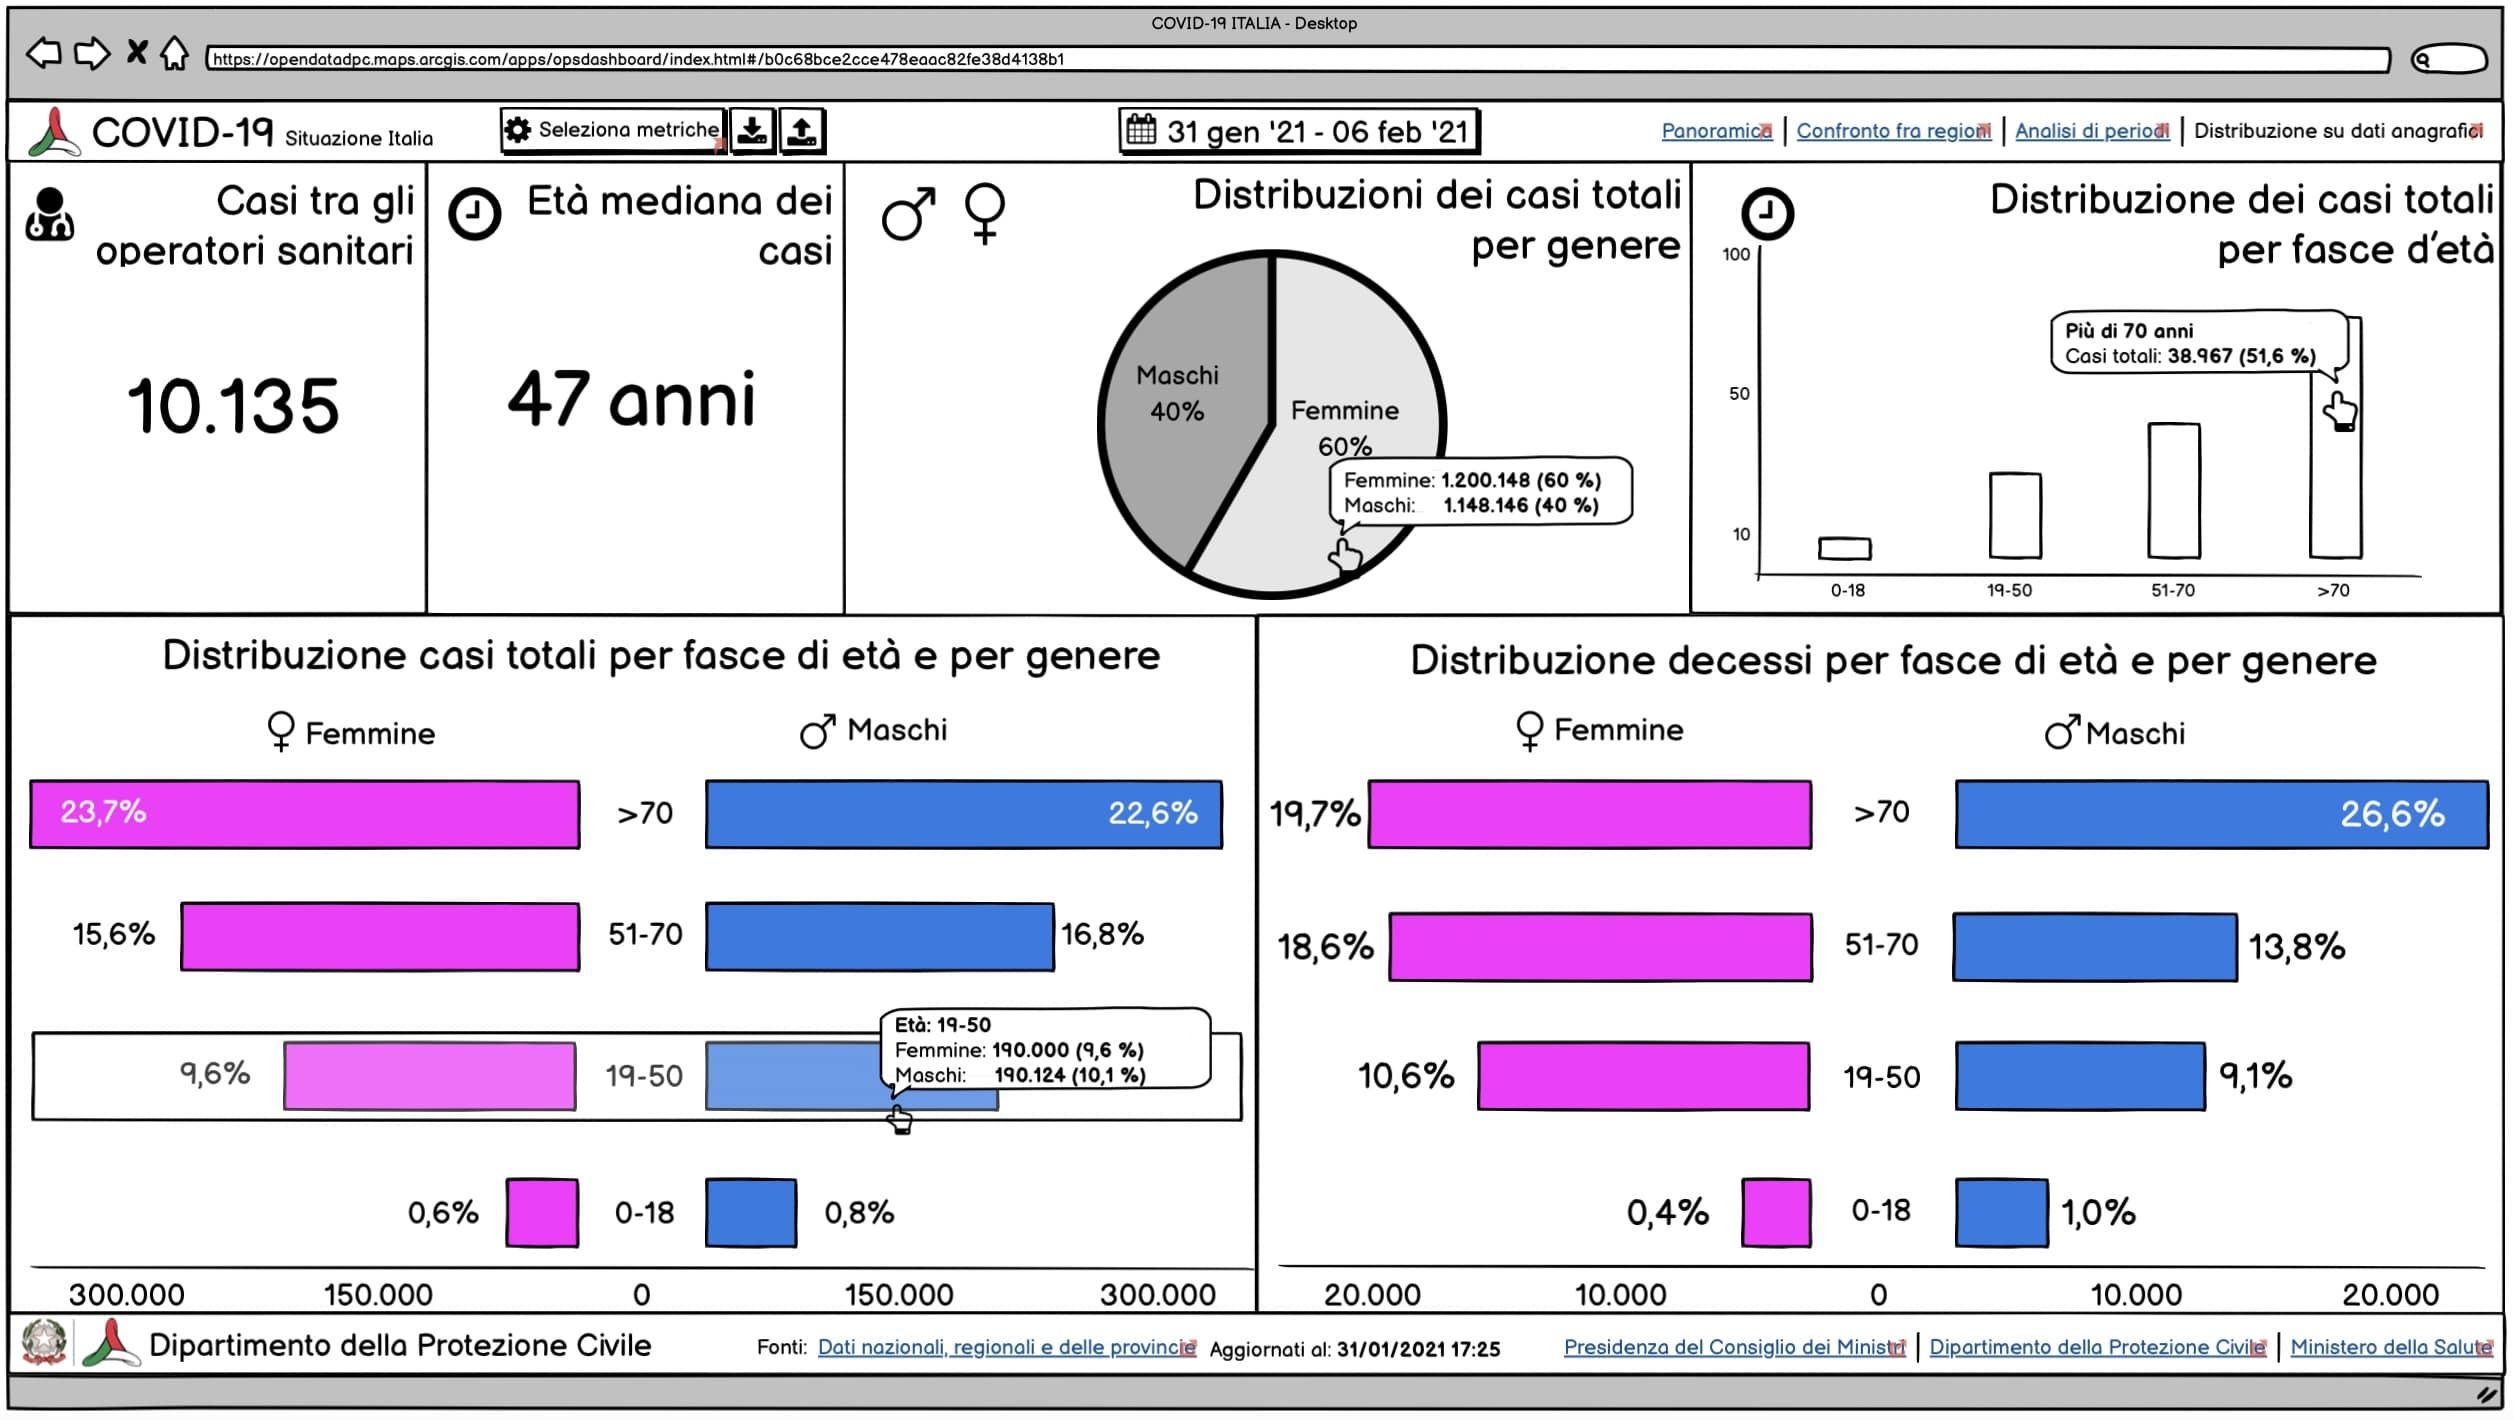
\includegraphics[width=1\columnwidth]{wireframes/distribuzione-dati-anagrafici}
    \caption{Schermata ``Distribuzione sui dati anagrafici''.}
    \label{fig:distribuzione-dati-anagrafici}
\end{figure}
La schermata ``Distribuzione sui dati anagrafici'' è raggiungibile dal link omonimo in alto a destra e permette di studiare la distribuzione dei casi totali e dei decessi su dati anagrafici, quali età, genere e categoria d'impiego: l'analisi è supportata da componenti grafiche quali box numerici, areogrammi e istogrammi.
\end{document}
